% Generated by Sphinx.
\def\sphinxdocclass{report}
\documentclass[a4,10pt,openany,oneside]{sphinxmanual}
\usepackage[utf8]{inputenc}
\DeclareUnicodeCharacter{00A0}{\nobreakspace}
\usepackage{cmap}
\usepackage[T1]{fontenc}
\usepackage[english]{babel}
\usepackage{times}
\usepackage[Bjarne]{fncychap}
\usepackage{longtable}
\usepackage{sphinx}
\usepackage{multirow}
\usepackage[left=0.75in, right=0.75in, top=1.0in, bottom=1.0in]{geometry}

\title{Blender User Manual}
\date{March 17, 2015}
\release{0.1}
\author{Blender Community}
\newcommand{\sphinxlogo}{}
\renewcommand{\releasename}{Release}
\makeindex

\makeatletter
\def\PYG@reset{\let\PYG@it=\relax \let\PYG@bf=\relax%
    \let\PYG@ul=\relax \let\PYG@tc=\relax%
    \let\PYG@bc=\relax \let\PYG@ff=\relax}
\def\PYG@tok#1{\csname PYG@tok@#1\endcsname}
\def\PYG@toks#1+{\ifx\relax#1\empty\else%
    \PYG@tok{#1}\expandafter\PYG@toks\fi}
\def\PYG@do#1{\PYG@bc{\PYG@tc{\PYG@ul{%
    \PYG@it{\PYG@bf{\PYG@ff{#1}}}}}}}
\def\PYG#1#2{\PYG@reset\PYG@toks#1+\relax+\PYG@do{#2}}

\expandafter\def\csname PYG@tok@mo\endcsname{\def\PYG@tc##1{\textcolor[rgb]{0.13,0.50,0.31}{##1}}}
\expandafter\def\csname PYG@tok@s1\endcsname{\def\PYG@tc##1{\textcolor[rgb]{0.25,0.44,0.63}{##1}}}
\expandafter\def\csname PYG@tok@vi\endcsname{\def\PYG@tc##1{\textcolor[rgb]{0.73,0.38,0.84}{##1}}}
\expandafter\def\csname PYG@tok@nl\endcsname{\let\PYG@bf=\textbf\def\PYG@tc##1{\textcolor[rgb]{0.00,0.13,0.44}{##1}}}
\expandafter\def\csname PYG@tok@cm\endcsname{\let\PYG@it=\textit\def\PYG@tc##1{\textcolor[rgb]{0.25,0.50,0.56}{##1}}}
\expandafter\def\csname PYG@tok@kp\endcsname{\def\PYG@tc##1{\textcolor[rgb]{0.00,0.44,0.13}{##1}}}
\expandafter\def\csname PYG@tok@s\endcsname{\def\PYG@tc##1{\textcolor[rgb]{0.25,0.44,0.63}{##1}}}
\expandafter\def\csname PYG@tok@kn\endcsname{\let\PYG@bf=\textbf\def\PYG@tc##1{\textcolor[rgb]{0.00,0.44,0.13}{##1}}}
\expandafter\def\csname PYG@tok@gr\endcsname{\def\PYG@tc##1{\textcolor[rgb]{1.00,0.00,0.00}{##1}}}
\expandafter\def\csname PYG@tok@nb\endcsname{\def\PYG@tc##1{\textcolor[rgb]{0.00,0.44,0.13}{##1}}}
\expandafter\def\csname PYG@tok@s2\endcsname{\def\PYG@tc##1{\textcolor[rgb]{0.25,0.44,0.63}{##1}}}
\expandafter\def\csname PYG@tok@mi\endcsname{\def\PYG@tc##1{\textcolor[rgb]{0.13,0.50,0.31}{##1}}}
\expandafter\def\csname PYG@tok@mf\endcsname{\def\PYG@tc##1{\textcolor[rgb]{0.13,0.50,0.31}{##1}}}
\expandafter\def\csname PYG@tok@gp\endcsname{\let\PYG@bf=\textbf\def\PYG@tc##1{\textcolor[rgb]{0.78,0.36,0.04}{##1}}}
\expandafter\def\csname PYG@tok@nc\endcsname{\let\PYG@bf=\textbf\def\PYG@tc##1{\textcolor[rgb]{0.05,0.52,0.71}{##1}}}
\expandafter\def\csname PYG@tok@il\endcsname{\def\PYG@tc##1{\textcolor[rgb]{0.13,0.50,0.31}{##1}}}
\expandafter\def\csname PYG@tok@kd\endcsname{\let\PYG@bf=\textbf\def\PYG@tc##1{\textcolor[rgb]{0.00,0.44,0.13}{##1}}}
\expandafter\def\csname PYG@tok@gi\endcsname{\def\PYG@tc##1{\textcolor[rgb]{0.00,0.63,0.00}{##1}}}
\expandafter\def\csname PYG@tok@err\endcsname{\def\PYG@bc##1{\setlength{\fboxsep}{0pt}\fcolorbox[rgb]{1.00,0.00,0.00}{1,1,1}{\strut ##1}}}
\expandafter\def\csname PYG@tok@o\endcsname{\def\PYG@tc##1{\textcolor[rgb]{0.40,0.40,0.40}{##1}}}
\expandafter\def\csname PYG@tok@si\endcsname{\let\PYG@it=\textit\def\PYG@tc##1{\textcolor[rgb]{0.44,0.63,0.82}{##1}}}
\expandafter\def\csname PYG@tok@ss\endcsname{\def\PYG@tc##1{\textcolor[rgb]{0.32,0.47,0.09}{##1}}}
\expandafter\def\csname PYG@tok@w\endcsname{\def\PYG@tc##1{\textcolor[rgb]{0.73,0.73,0.73}{##1}}}
\expandafter\def\csname PYG@tok@sx\endcsname{\def\PYG@tc##1{\textcolor[rgb]{0.78,0.36,0.04}{##1}}}
\expandafter\def\csname PYG@tok@m\endcsname{\def\PYG@tc##1{\textcolor[rgb]{0.13,0.50,0.31}{##1}}}
\expandafter\def\csname PYG@tok@ow\endcsname{\let\PYG@bf=\textbf\def\PYG@tc##1{\textcolor[rgb]{0.00,0.44,0.13}{##1}}}
\expandafter\def\csname PYG@tok@cs\endcsname{\def\PYG@tc##1{\textcolor[rgb]{0.25,0.50,0.56}{##1}}\def\PYG@bc##1{\setlength{\fboxsep}{0pt}\colorbox[rgb]{1.00,0.94,0.94}{\strut ##1}}}
\expandafter\def\csname PYG@tok@nt\endcsname{\let\PYG@bf=\textbf\def\PYG@tc##1{\textcolor[rgb]{0.02,0.16,0.45}{##1}}}
\expandafter\def\csname PYG@tok@cp\endcsname{\def\PYG@tc##1{\textcolor[rgb]{0.00,0.44,0.13}{##1}}}
\expandafter\def\csname PYG@tok@mh\endcsname{\def\PYG@tc##1{\textcolor[rgb]{0.13,0.50,0.31}{##1}}}
\expandafter\def\csname PYG@tok@vc\endcsname{\def\PYG@tc##1{\textcolor[rgb]{0.73,0.38,0.84}{##1}}}
\expandafter\def\csname PYG@tok@gt\endcsname{\def\PYG@tc##1{\textcolor[rgb]{0.00,0.27,0.87}{##1}}}
\expandafter\def\csname PYG@tok@se\endcsname{\let\PYG@bf=\textbf\def\PYG@tc##1{\textcolor[rgb]{0.25,0.44,0.63}{##1}}}
\expandafter\def\csname PYG@tok@na\endcsname{\def\PYG@tc##1{\textcolor[rgb]{0.25,0.44,0.63}{##1}}}
\expandafter\def\csname PYG@tok@go\endcsname{\def\PYG@tc##1{\textcolor[rgb]{0.20,0.20,0.20}{##1}}}
\expandafter\def\csname PYG@tok@nd\endcsname{\let\PYG@bf=\textbf\def\PYG@tc##1{\textcolor[rgb]{0.33,0.33,0.33}{##1}}}
\expandafter\def\csname PYG@tok@gd\endcsname{\def\PYG@tc##1{\textcolor[rgb]{0.63,0.00,0.00}{##1}}}
\expandafter\def\csname PYG@tok@sh\endcsname{\def\PYG@tc##1{\textcolor[rgb]{0.25,0.44,0.63}{##1}}}
\expandafter\def\csname PYG@tok@kt\endcsname{\def\PYG@tc##1{\textcolor[rgb]{0.56,0.13,0.00}{##1}}}
\expandafter\def\csname PYG@tok@no\endcsname{\def\PYG@tc##1{\textcolor[rgb]{0.38,0.68,0.84}{##1}}}
\expandafter\def\csname PYG@tok@sr\endcsname{\def\PYG@tc##1{\textcolor[rgb]{0.14,0.33,0.53}{##1}}}
\expandafter\def\csname PYG@tok@kc\endcsname{\let\PYG@bf=\textbf\def\PYG@tc##1{\textcolor[rgb]{0.00,0.44,0.13}{##1}}}
\expandafter\def\csname PYG@tok@kr\endcsname{\let\PYG@bf=\textbf\def\PYG@tc##1{\textcolor[rgb]{0.00,0.44,0.13}{##1}}}
\expandafter\def\csname PYG@tok@ne\endcsname{\def\PYG@tc##1{\textcolor[rgb]{0.00,0.44,0.13}{##1}}}
\expandafter\def\csname PYG@tok@bp\endcsname{\def\PYG@tc##1{\textcolor[rgb]{0.00,0.44,0.13}{##1}}}
\expandafter\def\csname PYG@tok@gs\endcsname{\let\PYG@bf=\textbf}
\expandafter\def\csname PYG@tok@c1\endcsname{\let\PYG@it=\textit\def\PYG@tc##1{\textcolor[rgb]{0.25,0.50,0.56}{##1}}}
\expandafter\def\csname PYG@tok@ni\endcsname{\let\PYG@bf=\textbf\def\PYG@tc##1{\textcolor[rgb]{0.84,0.33,0.22}{##1}}}
\expandafter\def\csname PYG@tok@gh\endcsname{\let\PYG@bf=\textbf\def\PYG@tc##1{\textcolor[rgb]{0.00,0.00,0.50}{##1}}}
\expandafter\def\csname PYG@tok@nv\endcsname{\def\PYG@tc##1{\textcolor[rgb]{0.73,0.38,0.84}{##1}}}
\expandafter\def\csname PYG@tok@gu\endcsname{\let\PYG@bf=\textbf\def\PYG@tc##1{\textcolor[rgb]{0.50,0.00,0.50}{##1}}}
\expandafter\def\csname PYG@tok@nn\endcsname{\let\PYG@bf=\textbf\def\PYG@tc##1{\textcolor[rgb]{0.05,0.52,0.71}{##1}}}
\expandafter\def\csname PYG@tok@vg\endcsname{\def\PYG@tc##1{\textcolor[rgb]{0.73,0.38,0.84}{##1}}}
\expandafter\def\csname PYG@tok@sb\endcsname{\def\PYG@tc##1{\textcolor[rgb]{0.25,0.44,0.63}{##1}}}
\expandafter\def\csname PYG@tok@sc\endcsname{\def\PYG@tc##1{\textcolor[rgb]{0.25,0.44,0.63}{##1}}}
\expandafter\def\csname PYG@tok@k\endcsname{\let\PYG@bf=\textbf\def\PYG@tc##1{\textcolor[rgb]{0.00,0.44,0.13}{##1}}}
\expandafter\def\csname PYG@tok@sd\endcsname{\let\PYG@it=\textit\def\PYG@tc##1{\textcolor[rgb]{0.25,0.44,0.63}{##1}}}
\expandafter\def\csname PYG@tok@nf\endcsname{\def\PYG@tc##1{\textcolor[rgb]{0.02,0.16,0.49}{##1}}}
\expandafter\def\csname PYG@tok@ge\endcsname{\let\PYG@it=\textit}
\expandafter\def\csname PYG@tok@c\endcsname{\let\PYG@it=\textit\def\PYG@tc##1{\textcolor[rgb]{0.25,0.50,0.56}{##1}}}

\def\PYGZbs{\char`\\}
\def\PYGZus{\char`\_}
\def\PYGZob{\char`\{}
\def\PYGZcb{\char`\}}
\def\PYGZca{\char`\^}
\def\PYGZam{\char`\&}
\def\PYGZlt{\char`\<}
\def\PYGZgt{\char`\>}
\def\PYGZsh{\char`\#}
\def\PYGZpc{\char`\%}
\def\PYGZdl{\char`\$}
\def\PYGZhy{\char`\-}
\def\PYGZsq{\char`\'}
\def\PYGZdq{\char`\"}
\def\PYGZti{\char`\~}
% for compatibility with earlier versions
\def\PYGZat{@}
\def\PYGZlb{[}
\def\PYGZrb{]}
\makeatother

\begin{document}

\maketitle
\tableofcontents
\phantomsection\label{index::doc}



\chapter{Installation}
\label{installation/index:installation}\label{installation/index:blender-vr-manual-contents}\label{installation/index::doc}

\section{Install BlenderVR}
\label{installation/installation:install-blendervr}\label{installation/installation::doc}
In order to install Blender-VR you need this guide.

\begin{notice}{note}{Note:}
If you need the full development setup make sure to follow the Development Environment guide.
\end{notice}


\subsection{Document Sections}
\label{installation/installation:document-sections}\begin{itemize}
\item {} 
{\hyperref[installation/installation:folder-structure]{Folder Structure}}

\item {} 
{\hyperref[installation/installation:acquiring-blender]{Acquiring Blender}}

\item {} 
{\hyperref[installation/installation:acquiring-blendervr]{Acquiring BlenderVR}}

\item {} 
{\hyperref[installation/installation:download-samples-scenes]{Download Samples Scenes}}

\item {} 
{\hyperref[installation/installation:install-dependecies]{Install dependecies}}

\item {} 
{\hyperref[installation/installation:quick-setup]{Quick Setup}}

\item {} 
{\hyperref[installation/installation:running]{Running}}

\end{itemize}


\subsection{Folder Structure}
\label{installation/installation:folder-structure}
After all the downloads and installations you should end up with the following folder structure. This is a recommendation, and it will be used as reference along this manual (the directory holding these files is  referred as \$INSTALL\_DIR in the next sections).

\code{//blender-vr/}
\emph{Blender-VR Source Code}

\code{//blender/}
\emph{Blender Binaries}

\code{//samples/}
\emph{Blender-VR Samples}

\code{//venv/}
\emph{Python Virtual Environment}


\subsection{Acquiring Blender}
\label{installation/installation:acquiring-blender}
Blender-VR requires \href{http://www.blender.org/download}{Blender 2.74} or newer.
Optionally you can use  a patched version of Blender 2.73a available here for all the supported platforms.
\begin{itemize}
\item {} 
\href{http://www.dalaifelinto.com/blendervr/ftp/blender-2.73-5c6ef95-OSX-10.6-x86\_64.zip}{Mac OSX 64 bit: Blender 2.73a Patched}. \footnote{
Requires Mac OSX 10.6+
}

\item {} 
\href{http://www.dalaifelinto.com/blendervr/ftp/https://builder.blender.org/download/blender-2.73-5c6ef95-win32.zip}{Windows 32 bit: Blender 2.73a Patched}. \footnote{
Compatible with Windows 8, 7, Vista. If Blender reports an error on startup, please install the \href{http://www.microsoft.com/en-us/download/details.aspx?id=40784}{Visual C++ 2013 Redistributable Package}.
}

\item {} 
\href{http://www.dalaifelinto.com/blendervr/ftp/blender-2.73-5c6ef95-win64.zip}{Windows 64 bit: Blender 2.73a Patched}. \footnotemark[2]

\item {} 
\href{http://www.dalaifelinto.com/blendervr/ftp/blender-2.73-5c6ef95-linux-glibc211-i686.tar.bz2}{Linux 32 bit: Blender 2.73a Patched}. \footnote{
Requires glibc 2.11. Suits most recent GNU/Linux distributions
}

\item {} 
\href{http://www.dalaifelinto.com/blendervr/ftp/blender-2.73-5c6ef95-linux-glibc211-x86\_64.tar.bz2}{Linux 64 bit: Blender 2.73a Patched}. \footnotemark[3]

\end{itemize}


\subsection{Acquiring BlenderVR}
\label{installation/installation:acquiring-blendervr}\begin{itemize}
\item {} 
\href{https://github.com/BlenderVR/blender-vr/archive/v1.0.zip}{Blender-VR Sources} (download and unzip in the top folder, rename it \textbf{blender-vr})

\end{itemize}


\subsection{Download Samples Scenes}
\label{installation/installation:download-samples-scenes}
Before getting started, you'll probably want to take a look at the available blenderVR ''.blend'' sample scenes.
\begin{itemize}
\item {} 
Download \href{https://github.com/BlenderVR/samples/archive/master.zip}{All Samples}

\end{itemize}

You can also download an individual sample folder. For that you will need \href{http://subversion.apache.org/}{SVN} or \href{http://tortoisesvn.net/}{SVN Tortoise} (Windows only).
To check which samples are available visit the \href{https://github.com/BlenderVR/samples.git}{Samples Repository}.

\begin{Verbatim}[commandchars=\\\{\}]
\PYG{n+nv}{\PYGZdl{} }\PYG{n+nb}{cd} \PYG{n+nv}{\PYGZdl{}INSTALL\PYGZus{}DIR}
\PYG{n+nv}{\PYGZdl{} }mkdir \PYGZhy{}p samples
\PYG{n+nv}{\PYGZdl{} }svn checkout https://github.com/BlenderVR/samples/trunk/simple samples/
\end{Verbatim}

(Or simply \emph{svn checkout} the required sample with SVN Tortoise).


\subsection{Install dependecies}
\label{installation/installation:install-dependecies}
Install those packages or make sure you have them in your system.


\subsubsection{All Time Mandatory}
\label{installation/installation:all-time-mandatory}\begin{itemize}
\item {} 
\href{https://www.python.org/downloads/release/python-343/}{Python 3.4}

\end{itemize}

\emph{Future developments will make the following packages optional:}
\begin{itemize}
\item {} 
\href{http://download.qt.io/archive/qt/4.8/4.8.6/}{QT 4.8}

\item {} 
\href{https://pip.pypa.io/en/latest/installing.html}{PIP} (the Python install should have installed pip, try to use it in the next Section before installing)

\end{itemize}

\begin{notice}{note}{Note:}
MacOS: open Qt.mpkg with mouse right click -\textgreater{} Open, to avoid popup window ``can't install, non identified developer''.
\end{notice}


\subsection{Quick Setup}
\label{installation/installation:quick-setup}
Type the following commands in your terminal. If you are in Windows we recommend you to use \href{https://technet.microsoft.com/en-us/scriptcenter/default}{Power Shell} or similar.

On OSX/Linux:

\begin{Verbatim}[commandchars=\\\{\}]
\PYG{n+nv}{\PYGZdl{} }\PYG{n+nb}{cd} \PYG{n+nv}{\PYGZdl{}INSTALL\PYGZus{}DIR}
\PYG{n+nv}{\PYGZdl{} }pip3 install virtualenv
\PYG{n+nv}{\PYGZdl{} }pyvenv venv
\PYG{n+nv}{\PYGZdl{} }\PYG{n+nb}{source }venv/bin/activate
\PYG{n+nv}{\PYGZdl{} }pip3 install \PYGZhy{}r blender\PYGZhy{}vr/requirements.txt
\PYG{n+nv}{\PYGZdl{} }pyside\PYGZus{}postinstall.py \PYGZhy{}install
\end{Verbatim}

\begin{notice}{note}{Note:}
MacOS: running these lines may popup window ``download the command line developer tools'', go for it.
\end{notice}

On Windows:

\begin{Verbatim}[commandchars=\\\{\}]
\PYG{n+nv}{\PYGZdl{} }\PYG{n+nb}{cd} \PYG{n+nv}{\PYGZdl{}INSTALL\PYGZus{}DIR}
\PYG{n+nv}{\PYGZdl{} }pip3 install virtualenv
\PYG{n+nv}{\PYGZdl{} }virtualenv venv
\PYG{n+nv}{\PYGZdl{} }.\PYG{l+s+se}{\PYGZbs{}v}env\PYG{l+s+se}{\PYGZbs{}S}cripts\PYG{l+s+se}{\PYGZbs{}a}ctivate
\PYG{n+nv}{\PYGZdl{} }pip3 install \PYGZhy{}r blender\PYGZhy{}vr\PYG{l+s+se}{\PYGZbs{}r}equirements.txt
\PYG{n+nv}{\PYGZdl{} }python3 .\PYG{l+s+se}{\PYGZbs{}v}env\PYG{l+s+se}{\PYGZbs{}S}cripts\PYG{l+s+se}{\PYGZbs{}p}yside\PYGZus{}postinstall.py \PYGZhy{}install
\PYG{n+nv}{\PYGZdl{} }python3 .\PYG{l+s+se}{\PYGZbs{}b}lender\PYGZhy{}vr\PYG{l+s+se}{\PYGZbs{}b}lenderVR
\end{Verbatim}

You may have to add the path to the python binary, e.g.

\begin{Verbatim}[commandchars=\\\{\}]
\PYGZdl{} [Environment]::SetEnvironmentVariable(\PYGZdq{}Path\PYGZdq{}, \PYGZdq{}\PYGZdl{}env:Path;C:\PYGZbs{}Python34\PYGZbs{};C:\PYGZbs{}Python34\PYGZbs{}Scripts\PYGZbs{}\PYGZdq{})
\end{Verbatim}

\emph{(For PowerShell to automatically add this path at startup, add this line to a file named e.g. profile.ps1 that you'll place in your WindowsPowerShell directory)}


\subsection{Running}
\label{installation/installation:running}
Type the following commands in your terminal. If you are in Windows we recommend you to use \href{https://technet.microsoft.com/en-us/scriptcenter/default}{Power Shell} or similar.

On OSX/Linux:

\begin{Verbatim}[commandchars=\\\{\}]
\PYG{n+nv}{\PYGZdl{} }\PYG{n+nb}{cd} \PYG{n+nv}{\PYGZdl{}INSTALL\PYGZus{}DIR}
\PYG{n+nv}{\PYGZdl{} }\PYG{n+nb}{source }venv/bin/activate
\PYG{n+nv}{\PYGZdl{} }./blender\PYGZhy{}vr/blenderVR
\end{Verbatim}

On Windows:

\begin{Verbatim}[commandchars=\\\{\}]
\PYG{n+nv}{\PYGZdl{} }\PYG{n+nb}{cd} \PYG{n+nv}{\PYGZdl{}INSTALL\PYGZus{}DIR}
\PYG{n+nv}{\PYGZdl{} }.\PYG{l+s+se}{\PYGZbs{}v}env\PYG{l+s+se}{\PYGZbs{}S}cripts\PYG{l+s+se}{\PYGZbs{}a}ctivate
\PYG{n+nv}{\PYGZdl{} }python3 .\PYG{l+s+se}{\PYGZbs{}b}lender\PYGZhy{}vr\PYG{l+s+se}{\PYGZbs{}b}lenderVR
\end{Verbatim}

You should now see the blenderVR window popping up (see figure below). Congratulations your installation was a success!
\begin{figure}[htbp]
\centering

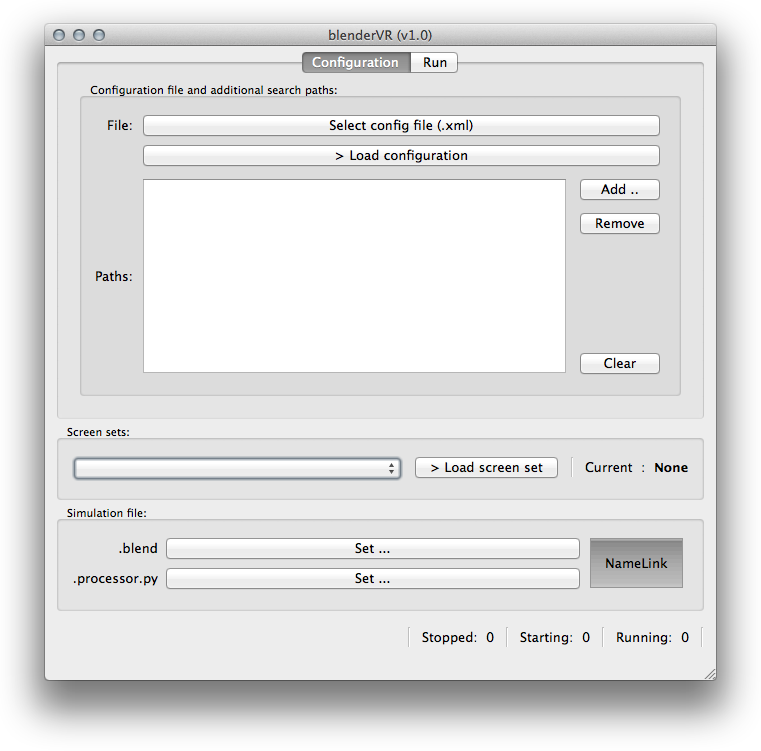
\includegraphics{user-interface-1.png}
\end{figure}

Once you are done running Blender-VR you can end the virtual environment running the command:

\begin{Verbatim}[commandchars=\\\{\}]
\PYG{n+nv}{\PYGZdl{} }deactivate
\end{Verbatim}

For your convenience it is recommended to create a bash script to help re-launching the Blender-VR environment.


\section{Install for Future blenderVR Developers}
\label{installation/development:install-for-future-blendervr-developers}\label{installation/development::doc}
This guide walks you over the basic steps of setting up a development environment for blenderVR.

\begin{notice}{note}{Note:}
For casual blenderVR users, please refer to the Install blenderVR page.
\end{notice}

The install is the same than described in Install blenderVR but for:
\begin{itemize}
\item {} 
git clone of the blenderVR repository, to freely modify and eventually commit your modifications.

\item {} 
svn/git clone of the blenderVR samples, to eventually add your own demo scenes to the blenderVR samples repository

\item {} 
manual compilation of Blender, if you need to modify its source code.

\end{itemize}

Most of the time you won't need to modify and rebuild Blender, so those instructions are specified separately.


\subsection{Document Sections}
\label{installation/development:document-sections}\begin{itemize}
\item {} 
Acquiring Blender

\item {} 
{\hyperref[installation/development:acquiring-blendervr]{Acquiring BlenderVR}}

\item {} 
{\hyperref[installation/development:download-samples-scenes]{Download Samples Scenes}}

\item {} 
{\hyperref[installation/development:id3]{Requirements}}

\item {} 
Quick Setup and Running

\end{itemize}


\subsection{Acquiring Blender}
\label{installation/development:acquiring-blender}
Blender-VR requires a vanilla Blender 2.74 or newer.

If you ever need to modify and rebuild Blender for further customizations, please consult the \href{http://wiki.blender.org/index.php/Dev:Doc/Building\_Blender}{Blender's official documentation}.

Else, download the sources provided in Acquiring Blender.


\subsection{Acquiring BlenderVR}
\label{installation/development:acquiring-blendervr}
To download the latest blenderVR git version (master HEAD):

\begin{Verbatim}[commandchars=\\\{\}]
\PYG{n+nv}{\PYGZdl{} }git clone https://github.com/BlenderVR/blender\PYGZhy{}vr.git
\end{Verbatim}

If you do not intend to modify blenderVR source code, simply download the \href{https://github.com/BlenderVR/blender-vr/archive/v1.0.zip}{Blender-VR Sources} zipfile.


\subsection{Download Samples Scenes}
\label{installation/development:download-samples-scenes}
Regarding blenderVR samples, Git is not a good system to work on binary files, so it's recommended to use the SVN protocol to interact with the samples repository instead:

\begin{Verbatim}[commandchars=\\\{\}]
\PYG{n+nv}{\PYGZdl{} }\PYG{n+nb}{cd} \PYG{n+nv}{\PYGZdl{}INSTALL\PYGZus{}DIR}
\PYG{n+nv}{\PYGZdl{} }svn checkout https://github.com/BlenderVR/samples
\end{Verbatim}

Or for an individual sample folder:

\begin{Verbatim}[commandchars=\\\{\}]
\PYG{n+nv}{\PYGZdl{} }svn checkout https://github.com/BlenderVR/samples/trunk/simple
\end{Verbatim}

Alternatively if you want to access the repository via GIT you can do:

\begin{Verbatim}[commandchars=\\\{\}]
\PYGZdl{} cd \PYGZdl{}INSTALL\PYGZus{}DIR
\PYGZdl{} git clone https://github.com/BlenderVR/samples.git
\end{Verbatim}


\subsection{Requirements}
\label{installation/development:requirements}\phantomsection\label{installation/development:id3}
Install those packages or make sure you have them in your system.


\subsubsection{All Time Mandatory}
\label{installation/development:all-time-mandatory}\begin{itemize}
\item {} 
\href{http://git-scm.com/}{GIT}

\item {} 
\href{https://www.python.org/downloads/release/python-343/}{Python 3.4}

\end{itemize}


\subsubsection{Required for Interface Development}
\label{installation/development:required-for-interface-development}
\emph{At this moment the following packages are always required, but the plans are to make them optional.}
\begin{itemize}
\item {} 
\href{https://pip.pypa.io/en/latest/installing.html}{PIP}

\item {} 
\href{http://download.qt.io/archive/qt/4.8/4.8.6/}{QT 4.8}

\end{itemize}


\subsection{Quick Setup and Running}
\label{installation/development:quick-setup-and-running}
see Quick Setup and Running in the Install blenderVR Section.


\chapter{First Run}
\label{first-run:first-run}\label{first-run::doc}
\begin{notice}{note}{Note:}
After the installation you should make sure everything is working before going on your own. For this first run you will need at least the basic sample from the samples repository.
\end{notice}


\section{Document Sections}
\label{first-run:document-sections}\begin{itemize}
\item {} 
{\hyperref[first-run:launch-blender-vr]{Launch Blender-VR}}

\item {} 
{\hyperref[first-run:open-the-simulation-file]{Open the Simulation File}}

\item {} 
{\hyperref[first-run:edit-the-configuration-file]{Edit the Configuration File}}

\item {} 
{\hyperref[first-run:run]{Run}}

\end{itemize}


\section{Launch Blender-VR}
\label{first-run:launch-blender-vr}
Start by opening the blenderVR GUI (see Running BlenderVR in the Install section). Although in the future you can launch it via a shortcut, for the first run it's better to do it via command-line, to catch any unexpected error.
It is advised to understand how to manipulate the User Interface before going any further.


\section{Open the Simulation File}
\label{first-run:open-the-simulation-file}
In the Simulation File select the \code{basic.blend} file. Mark \code{NameLink} for the \code{basic.processor.py} to be automatically selected as the Processor File.


\section{Edit the Configuration File}
\label{first-run:edit-the-configuration-file}
You now need a valid Configuration File to run Blender-VR. Make sure to follow the correct instructions and set a correct \code{blender} and \code{blenderplayer} paths.

Remember to select and load the configuration file.

\begin{notice}{note}{Note:}
For the initial test it's recommended to create a single screen with a mono buffer setup.
\end{notice}


\section{Run}
\label{first-run:run}
If there are no errors in the configuration tab, change to the \code{Run} tab and hit Start .

Congratulations, you can now try the other sample files, configuration options and finally bring your own \code{.blend} files into Blender-VR.


\chapter{How to Use}
\label{components/index:how-to-use}\label{components/index::doc}

\section{User Interface}
\label{components/user-interface:user-interface}\label{components/user-interface::doc}
We dissociate the \emph{controlling interface} from the \emph{virtual environment}.

The \emph{controlling interface} (here called \code{console}) is the graphical user interface (GUI) that controls Blender-VR. The \emph{virtual environment} is the part of the simulation that runs on each node inside \code{blenderplayer}.

To simplify, the \code{console} is run by the user, use PySide but cannot import \code{bge} python module whereas the \emph{virtual environment} is run by \code{blenderplayer}, don't have any GUI and can import \code{bge} python module.

From the processor file perspective there is even a third mode, the \code{update loader}. This mode is a glue between the previous ones. In the \code{update loader} the \code{.blend} file is changed on-the-fly so when it runs into the \code{virtual environment} it interacts with the \code{console} and with eventual interaction devices.


\subsection{Document Sections}
\label{components/user-interface:document-sections}\begin{itemize}
\item {} 
{\hyperref[components/user-interface:console]{Console}}
\begin{itemize}
\item {} 
Configuration File

\item {} 
{\hyperref[components/user-interface:active-screen-set]{Active Screen Set}}

\item {} 
{\hyperref[components/user-interface:simulation-file]{Simulation File}}

\item {} 
{\hyperref[components/user-interface:start-stop]{Start/Stop}}

\item {} 
{\hyperref[components/user-interface:debug-window-per-screen]{Debug Window per Screen}}

\item {} 
{\hyperref[components/user-interface:standard-error-outputs]{Standard/Error Outputs}}

\item {} 
{\hyperref[components/user-interface:log-level]{Log Level}}

\end{itemize}

\item {} 
{\hyperref[components/user-interface:daemons]{Daemons}}

\end{itemize}


\subsection{Console}
\label{components/user-interface:console}
The so called \code{console} is the GUI of Blender-VR. It allows you to choose the configuration file, the screen set to use, the simulation file (.blend) or to run blenderVR.
\begin{figure}[htbp]
\centering
\capstart

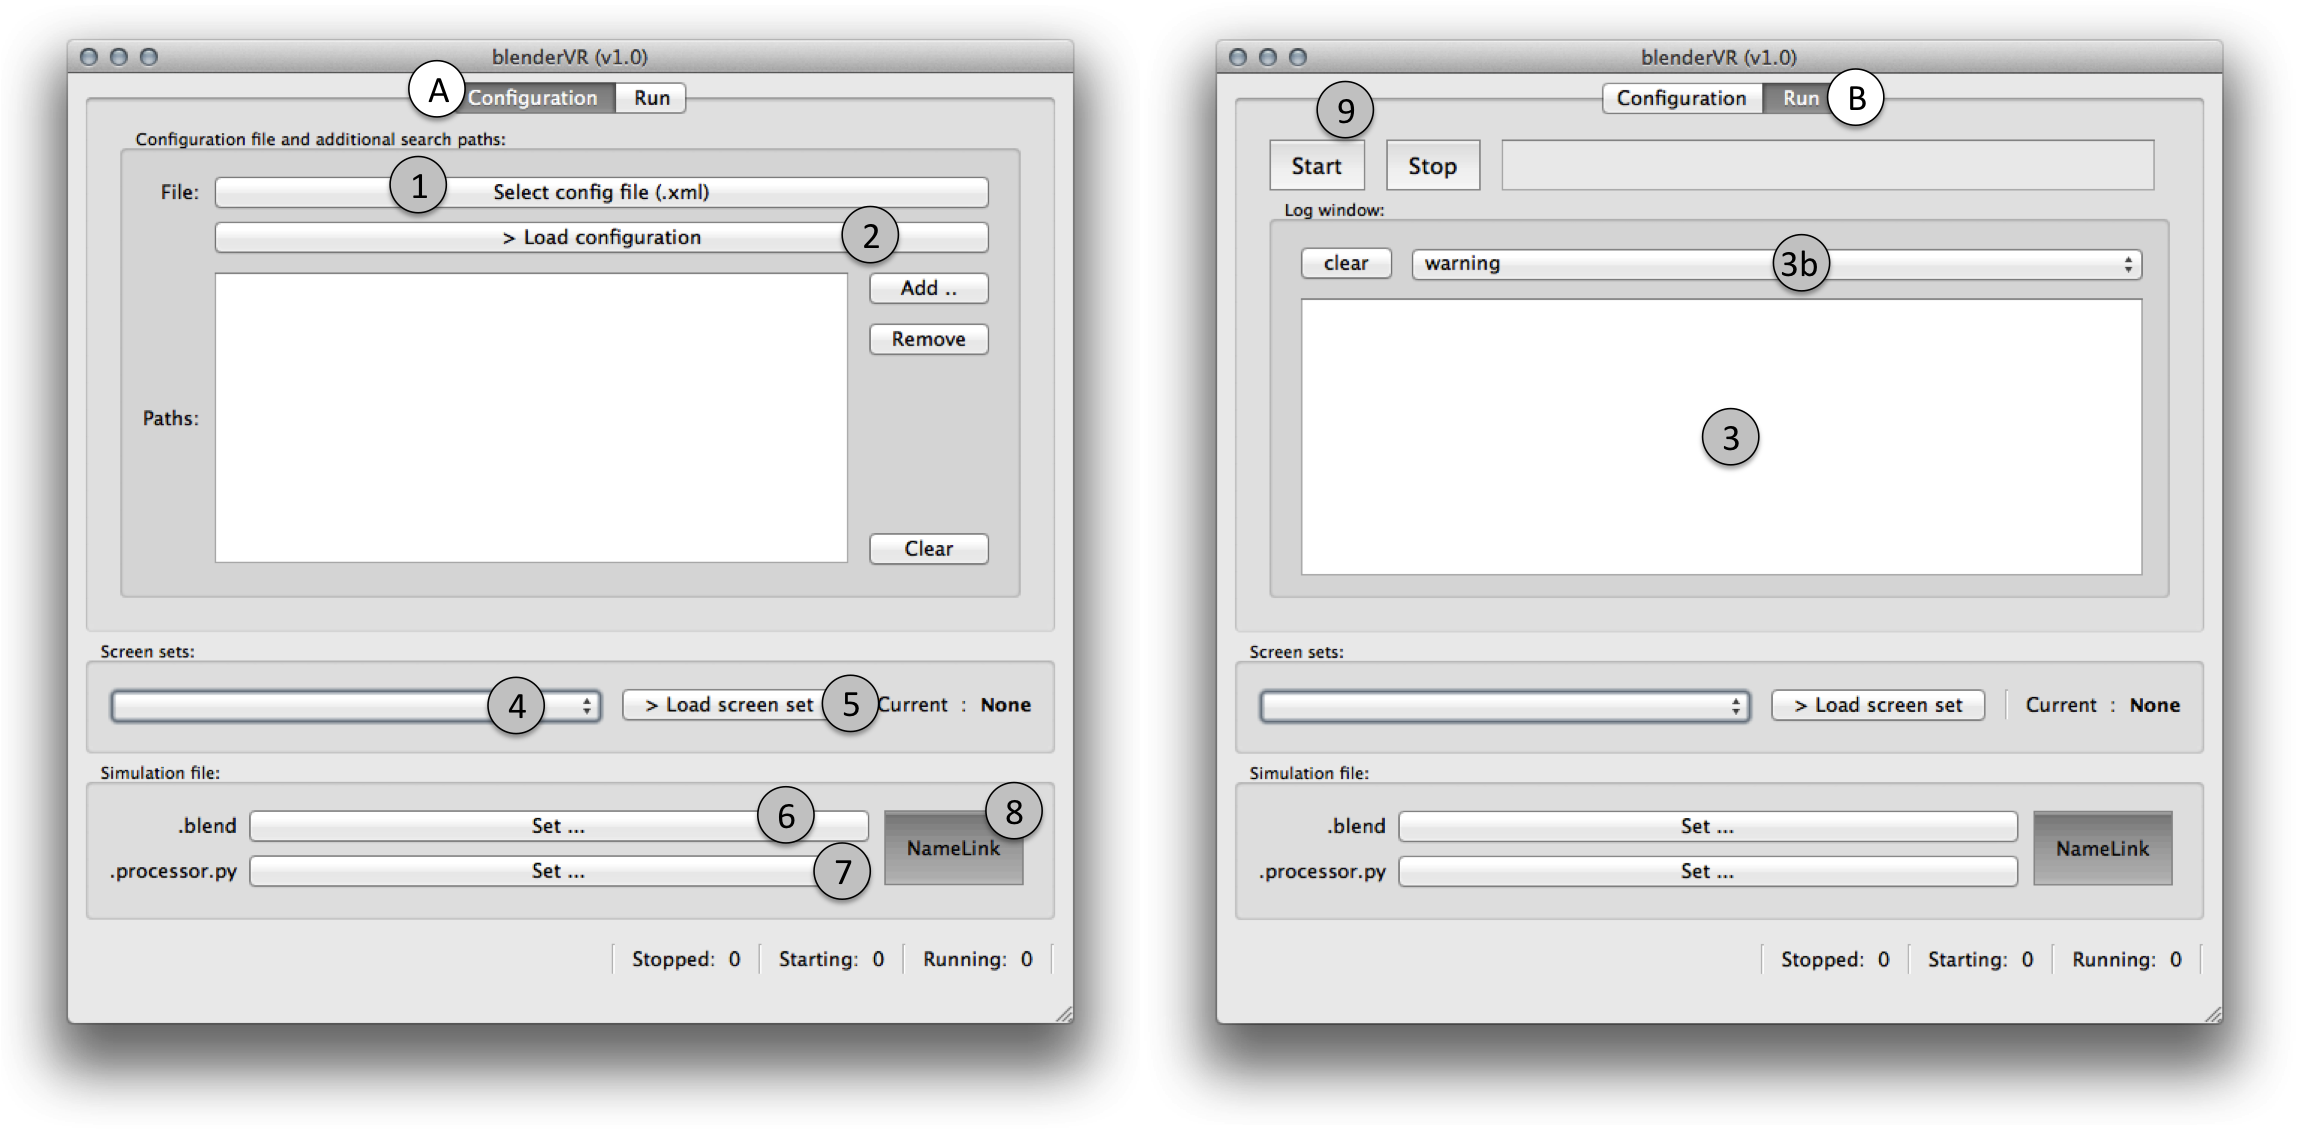
\includegraphics{user-interface-1and2.png}
\caption{Console Graphical User Interface (left: \code{Configuration} tab, right: \code{Run} tab)}\end{figure}

By default, the \code{console} does not ``know'' anything. You have to manually set configuration file, active screen-set, simulation file ... However, it stores these relevant informations in its internal data store path (see above). So you have to set these informations the first time you run Blender-VR and they remain active (across different running) until you change it with the GUI.


\subsubsection{Configuration File}
\label{components/user-interface:configuration-file}
You can specify the \code{XML} file inside the \code{configuration} tab (A-1). Don't forget to click on \code{\textgreater{} Load configuration} (A-2) to ask Blender-VR to read the configuration file (and store it inside its internal data file) ! You should go to \code{run} tab (B) and select \code{debug} (3b) inside the log window (3) to see if there is bug inside your configuration file.


\subsubsection{Active Screen Set}
\label{components/user-interface:active-screen-set}
You can choose any screen set (4) that is defined inside your \code{XML} configuration file. You also must click on \code{\textgreater{} Load screen set} (5) to make it active (and register it for further Blender-VR usage). The current active screen set is displayed on the right.


\subsubsection{Simulation File}
\label{components/user-interface:simulation-file}
Here, you must select the \code{.blend} file you want to load (6). For the beginning, you should try the \code{basic.blend}, that you can get from the samples repository. You can manually select a processor file (7) or activate the \code{NameLink} (8) for blenderVR to automatically look for a \textless{}name\_of\_blender\_scene\textgreater{}.processor.py file in the directory of the .blend  file. You will learn to create your own .blend scenes and processor files via the samples and going though the \href{http://blender-vr.readthedocs.org}{blenderVR API}.


\subsubsection{Start/Stop}
\label{components/user-interface:start-stop}
When everything is defined you can try to start/stop (9) by going to the \code{Run} tab. Have a look at the main log window below the Start and the Stop buttons.


\subsubsection{Debug Window per Screen}
\label{components/user-interface:debug-window-per-screen}
Once the configuration file and the screen set are loaded, you can also have a look at the per screen log window : top screen menu \code{Windows} \textgreater{} \code{Screens} and select the screen that you want to debug. We suggest, at the beginning, to debug your XML configuration file, to set it to debug mode and activate \code{Standard output} and \code{Error output}.
\begin{figure}[htbp]
\centering
\capstart

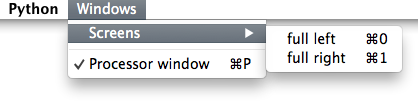
\includegraphics{select-screen.png}
\caption{Top screen \code{Windows} menu.}\end{figure}
\begin{figure}[htbp]
\centering
\capstart

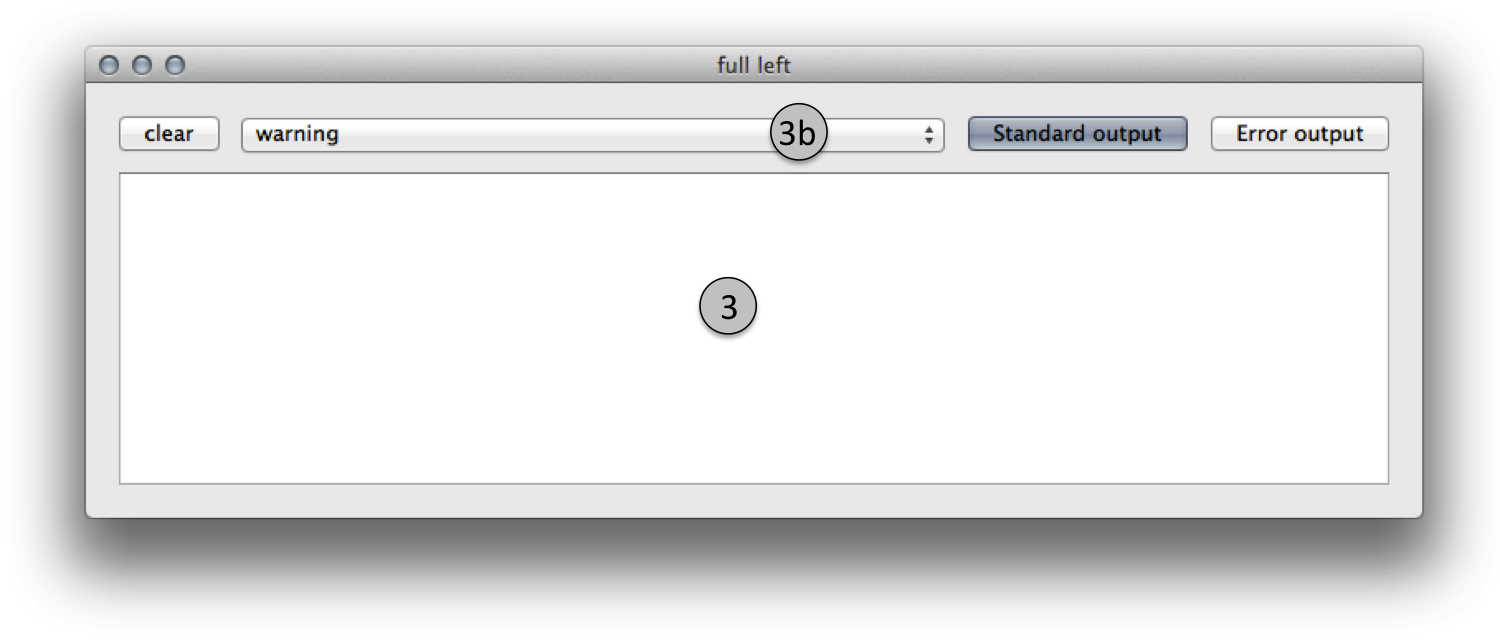
\includegraphics{screen-window.png}
\caption{Screen window for screen named \code{full left} in the configuration file.}\end{figure}


\subsubsection{Standard/Error Outputs}
\label{components/user-interface:standard-error-outputs}
They will display \code{stdout} and \code{stderr} of the instance of blenderplayer. Thus, you will see if there is a bug while running it. When blenderplayer runs correctly, you should disable these options.


\subsubsection{Log Level}
\label{components/user-interface:log-level}
The log level (3b) is usefull when blenderplayer runs properly. It can display errors of your processor file in the log window (3).


\subsection{Daemons}
\label{components/user-interface:daemons}
The \code{console} use one daemon per screen. The daemon is a python script that:
\begin{itemize}
\item {} 
Connects by network to the \code{console} and interact with it.

\item {} 
Start the instance of blenderplayer (for the ``virtual environment'') when required.

\item {} 
Catch blenderplayer's \code{stdout} and \code{stderr} to address them to the \code{console} if requested.

\item {} 
Kill blenderplayer if the ``virtual environment'' don't gently stop on \code{console} request.

\item {} 
. . .

\end{itemize}

In other words, the daemon manages blenderplayer. It runs on the computer that will run the blenderplayer instance.

Under Linux, this daemon becomes a real UNIX daemon (fork, close input and output ...).

\begin{notice}{note}{Note:}
The daemon script is included inside Blender-VR - you don't have to tweak it.
\end{notice}


\section{Processor File}
\label{components/processor-file:processor-file}\label{components/processor-file::doc}
We want to reduce the impact of blenderVR on the blender file (\code{.blend}).
For instance, all the interactions issued from the plugins (VRPN, OSC ...) don't have to be defined inside the \code{.blend} file, since they do not exists outside blenderVR development frame.
Moreover, elements to synchronize interaction from master to slaves cannot be defined inside \code{.blend} file.

Blender-VR thus introduces the notion of processor file. It is a Python file associated with the \code{.blend} that contains all the interactions required to use the \code{.blend} file within blenderVR.
By default (and you should not change it) this file is in the same folder than the \code{.blend} file and its name is the name of the blender file minus \code{.blend}, but post-fixed by \code{.processor.py}. For instance, the processor file of \code{simple.blend} is \code{simple.processor.py}.

Refer to the \href{http://blender-vr.readthedocs.org}{Complete API} for all the available commands and funcionality.


\subsection{Document Sections}
\label{components/processor-file:document-sections}\begin{itemize}
\item {} 
{\hyperref[components/processor-file:minimal-processor-file]{Minimal Processor File}}

\item {} 
{\hyperref[components/processor-file:basic-processor-file]{Basic Processor File}}

\item {} 
{\hyperref[components/processor-file:debugging-processor-through-log-messages]{Debugging Processor Through Log Messages}}

\item {} 
{\hyperref[components/processor-file:keyboard-and-mouse]{Keyboard and Mouse}}

\item {} 
{\hyperref[components/processor-file:choose-objects-to-synchronize]{Choose Objects to Synchronize}}

\item {} 
{\hyperref[components/processor-file:processor-inheritance]{Processor Inheritance}}

\item {} 
{\hyperref[components/processor-file:master-slaves-communication]{Master-Slaves Communication}}

\item {} 
{\hyperref[components/processor-file:stream-processor-as-synchronized-object]{Stream: Processor as Synchronized Object}}

\item {} 
{\hyperref[components/processor-file:one-shot-specifically-send-a-data]{One-Shot: Specifically Send a Data}}

\item {} 
{\hyperref[components/processor-file:run-method]{Run() Method}}

\item {} 
{\hyperref[components/processor-file:console-virtual-environment-communication]{Console-``Virtual Environment'' Communication}}

\end{itemize}


\subsection{Minimal Processor File}
\label{components/processor-file:minimal-processor-file}
The minimal processor file contains:

\begin{Verbatim}[commandchars=\\\{\}]
\PYG{k+kn}{import} \PYG{n+nn}{blendervr}

\PYG{k}{if} \PYG{n}{blendervr}\PYG{o}{.}\PYG{n}{is\PYGZus{}virtual\PYGZus{}environment}\PYG{p}{(}\PYG{p}{)}\PYG{p}{:}
    \PYG{k}{class} \PYG{n+nc}{Processor}\PYG{p}{(}\PYG{n}{blendervr}\PYG{o}{.}\PYG{n}{processor}\PYG{o}{.}\PYG{n}{getProcessor}\PYG{p}{(}\PYG{p}{)}\PYG{p}{)}\PYG{p}{:}
        \PYG{k}{def} \PYG{n+nf}{\PYGZus{}\PYGZus{}init\PYGZus{}\PYGZus{}}\PYG{p}{(}\PYG{n+nb+bp}{self}\PYG{p}{,} \PYG{n}{parent}\PYG{p}{)}\PYG{p}{:}
            \PYG{n+nb}{super}\PYG{p}{(}\PYG{n}{Processor}\PYG{p}{,} \PYG{n+nb+bp}{self}\PYG{p}{)}\PYG{o}{.}\PYG{n}{\PYGZus{}\PYGZus{}init\PYGZus{}\PYGZus{}}\PYG{p}{(}\PYG{n}{parent}\PYG{p}{)}

\PYG{k}{elif} \PYG{n}{blendervr}\PYG{o}{.}\PYG{n}{is\PYGZus{}console}\PYG{p}{(}\PYG{p}{)}\PYG{p}{:}
    \PYG{k}{class} \PYG{n+nc}{Processor}\PYG{p}{(}\PYG{n}{blendervr}\PYG{o}{.}\PYG{n}{processor}\PYG{o}{.}\PYG{n}{getProcessor}\PYG{p}{(}\PYG{p}{)}\PYG{p}{)}\PYG{p}{:}
        \PYG{k}{def} \PYG{n+nf}{\PYGZus{}\PYGZus{}init\PYGZus{}\PYGZus{}}\PYG{p}{(}\PYG{n+nb+bp}{self}\PYG{p}{,} \PYG{n}{console}\PYG{p}{)}\PYG{p}{:}
            \PYG{n+nb}{super}\PYG{p}{(}\PYG{n}{Processor}\PYG{p}{,} \PYG{n+nb+bp}{self}\PYG{p}{)}\PYG{o}{.}\PYG{n}{\PYGZus{}\PYGZus{}init\PYGZus{}\PYGZus{}}\PYG{p}{(}\PYG{n}{console}\PYG{p}{)}
\end{Verbatim}


\subsection{Basic Processor File}
\label{components/processor-file:basic-processor-file}
Unlike the {\hyperref[components/processor-file:minimum-processor-file]{Minimum Processor File}}, this one actually does something (in this case it syncronizes all the objects between the master and the slaves. This is file is fully explained in the \href{http://blender-vrreadthedocs.org/processor-file/examples.html\#basic-example}{Basic Example} of the Blender-vR API.

\begin{Verbatim}[commandchars=\\\{\}]
\PYG{k+kn}{import} \PYG{n+nn}{blendervr}

\PYG{k}{if} \PYG{n}{blendervr}\PYG{o}{.}\PYG{n}{is\PYGZus{}virtual\PYGZus{}environment}\PYG{p}{(}\PYG{p}{)}\PYG{p}{:}
    \PYG{k+kn}{import} \PYG{n+nn}{bge}

    \PYG{k}{class} \PYG{n+nc}{Processor}\PYG{p}{(}\PYG{n}{blendervr}\PYG{o}{.}\PYG{n}{processor}\PYG{o}{.}\PYG{n}{getProcessor}\PYG{p}{(}\PYG{p}{)}\PYG{p}{)}\PYG{p}{:}
        \PYG{k}{def} \PYG{n+nf}{\PYGZus{}\PYGZus{}init\PYGZus{}\PYGZus{}}\PYG{p}{(}\PYG{n+nb+bp}{self}\PYG{p}{,} \PYG{n}{parent}\PYG{p}{)}\PYG{p}{:}
            \PYG{n+nb}{super}\PYG{p}{(}\PYG{n}{Processor}\PYG{p}{,} \PYG{n+nb+bp}{self}\PYG{p}{)}\PYG{o}{.}\PYG{n}{\PYGZus{}\PYGZus{}init\PYGZus{}\PYGZus{}}\PYG{p}{(}\PYG{n}{parent}\PYG{p}{)}

            \PYG{k}{if} \PYG{n+nb+bp}{self}\PYG{o}{.}\PYG{n}{blenderVR}\PYG{o}{.}\PYG{n}{isMaster}\PYG{p}{(}\PYG{p}{)}\PYG{p}{:}
                \PYG{n+nb+bp}{self}\PYG{o}{.}\PYG{n}{blenderVR}\PYG{o}{.}\PYG{n}{getSceneSynchronizer}\PYG{p}{(}\PYG{p}{)}\PYG{o}{.}\PYGZbs{}
                        \PYG{n}{getItem}\PYG{p}{(}\PYG{n}{bge}\PYG{o}{.}\PYG{n}{logic}\PYG{p}{)}\PYG{o}{.}\PYG{n}{activate}\PYG{p}{(}\PYG{n+nb+bp}{True}\PYG{p}{,} \PYG{n+nb+bp}{True}\PYG{p}{)}

\PYG{k}{elif} \PYG{n}{blendervr}\PYG{o}{.}\PYG{n}{is\PYGZus{}creating\PYGZus{}loader}\PYG{p}{(}\PYG{p}{)}\PYG{p}{:}
    \PYG{k+kn}{import} \PYG{n+nn}{bpy}

    \PYG{k}{class} \PYG{n+nc}{Processor}\PYG{p}{(}\PYG{n}{blendervr}\PYG{o}{.}\PYG{n}{processor}\PYG{o}{.}\PYG{n}{getProcessor}\PYG{p}{(}\PYG{p}{)}\PYG{p}{)}\PYG{p}{:}
        \PYG{k}{def} \PYG{n+nf}{\PYGZus{}\PYGZus{}init\PYGZus{}\PYGZus{}}\PYG{p}{(}\PYG{n+nb+bp}{self}\PYG{p}{,} \PYG{n}{creator}\PYG{p}{)}\PYG{p}{:}
            \PYG{n+nb}{super}\PYG{p}{(}\PYG{n}{Processor}\PYG{p}{,} \PYG{n+nb+bp}{self}\PYG{p}{)}\PYG{o}{.}\PYG{n}{\PYGZus{}\PYGZus{}init\PYGZus{}\PYGZus{}}\PYG{p}{(}\PYG{n}{creator}\PYG{p}{)}

\PYG{k}{elif} \PYG{n}{blendervr}\PYG{o}{.}\PYG{n}{is\PYGZus{}console}\PYG{p}{(}\PYG{p}{)}\PYG{p}{:}
    \PYG{k}{class} \PYG{n+nc}{Processor}\PYG{p}{(}\PYG{n}{blendervr}\PYG{o}{.}\PYG{n}{processor}\PYG{o}{.}\PYG{n}{getProcessor}\PYG{p}{(}\PYG{p}{)}\PYG{p}{)}\PYG{p}{:}
        \PYG{k}{def} \PYG{n+nf}{\PYGZus{}\PYGZus{}init\PYGZus{}\PYGZus{}}\PYG{p}{(}\PYG{n+nb+bp}{self}\PYG{p}{,} \PYG{n}{console}\PYG{p}{)}\PYG{p}{:}
            \PYG{k}{global} \PYG{n}{try\PYGZus{}wait\PYGZus{}user\PYGZus{}name}\PYG{p}{,} \PYG{n}{try\PYGZus{}chooser}\PYG{p}{,} \PYG{n}{try\PYGZus{}console\PYGZus{}arc\PYGZus{}balls}
            \PYG{n+nb}{super}\PYG{p}{(}\PYG{n}{Processor}\PYG{p}{,} \PYG{n+nb+bp}{self}\PYG{p}{)}\PYG{o}{.}\PYG{n}{\PYGZus{}\PYGZus{}init\PYGZus{}\PYGZus{}}\PYG{p}{(}\PYG{n}{console}\PYG{p}{)}

        \PYG{k}{def} \PYG{n+nf}{useLoader}\PYG{p}{(}\PYG{n+nb+bp}{self}\PYG{p}{)}\PYG{p}{:}
            \PYG{k}{return} \PYG{n+nb+bp}{True}
\end{Verbatim}


\subsection{Debugging Processor Through Log Messages}
\label{components/processor-file:debugging-processor-through-log-messages}
As you have probably seen in Debug window per screen , the output of blenderplayer is not displayed by default in the console during Blender-VR runs.

Thus, you cannot use basic \code{print} python commands to help you while debugging.

You should instead use the Blender-VR standard logger usable inside any blenderVR object (due to inheritance):

\begin{Verbatim}[commandchars=\\\{\}]
\PYG{n+nb+bp}{self}\PYG{o}{.}\PYG{n}{logger}\PYG{o}{.}\PYG{n}{debug}\PYG{p}{(}\PYG{l+s}{\PYGZdq{}}\PYG{l+s}{blah blah ...}\PYG{l+s}{\PYGZdq{}}\PYG{p}{)}
\end{Verbatim}

\emph{blah blah ...} is whatever you want, comma separated, as long as there is a ``stringification'' method (\code{\_\_str\_\_}) for each element.
The \href{http://blender-vr.readthedocs.org/modules/rst/blendervr.tools.logger.html?highlight=logger\#module-blendervr.tools.logger}{logger} object inherits from python \code{login} module. Thus, you can replace \code{debug} by \code{info}, \code{warning}, \code{error}, \code{critical}. Depending on the log window level selection (see the screen window of the \code{Run} tab of the Console), you will see your message or not.

You can also use \href{http://blender-vr.readthedocs.org/modules/rst/blendervr.tools.logger.html?highlight=log\_traceback\#blendervr.tools.logger.Logger.log\_traceback}{self.logger.log\_traceback(False)} to display the traceback of your program. \code{True} in parenthesis means an error, then Blender-VR will stop running in ``Virtual Environment''. This traceback is available inside as well as outside an exception.

There is also \href{http://blender-vr.readthedocs.org/modules/rst/blendervr.tools.logger.html?highlight=log\_position\#blendervr.tools.logger.Logger.log\_position}{self.logger.log\_position()} that simply displays the position of the calling method in \code{debug} level.


\subsection{Keyboard and Mouse}
\label{components/processor-file:keyboard-and-mouse}
You can get access to keyboard and mouse information of the master node by defining the \href{http://blender-vr.readthedocs.org/modules/rst/blendervr.processor.base.html?highlight=keyboardandmouse\#blendervr.processor.base.Processor.keyboardAndMouse}{keyboardAndMouse} method. The \code{info} provided has the same format than any provided through the VRPN plugin.

You can use a \href{http://blender-vr.readthedocs.org/modules/rst/blendervr.tools.logger.html?highlight=logger\#module-blendervr.tools.logger}{logger} to see what is contained inside the \code{info} argument. You can also have a look at the \code{simple.processor.py} file inside \code{simple} sample folder to get an example of how to use this method.


\subsection{Choose Objects to Synchronize}
\label{components/processor-file:choose-objects-to-synchronize}
By default, Blender-VR doesn't synchronize scene objects (blacklisting for efficiency issues). You must specify the elements you want to synchronize by explicitly flagging the objects to synchronize by the master node:

\begin{Verbatim}[commandchars=\\\{\}]
\PYG{c}{\PYGZsh{} synchronizer.objects.getItem(enable, recursive = True)}
\PYG{c}{\PYGZsh{} synchronizer.objects.item\PYGZus{}base.Base.activate(enable, recursive = True)}
\PYG{k}{if} \PYG{n+nb+bp}{self}\PYG{o}{.}\PYG{n}{blenderVR}\PYG{o}{.}\PYG{n}{isMaster}\PYG{p}{(}\PYG{p}{)}\PYG{p}{:}
   \PYG{n+nb+bp}{self}\PYG{o}{.}\PYG{n}{blenderVR}\PYG{o}{.}\PYG{n}{getSceneSynchronizer}\PYG{p}{(}\PYG{p}{)}\PYG{o}{.}\PYG{n}{getItem}\PYG{p}{(}\PYG{n}{bge}\PYG{o}{.}\PYG{n}{logic}\PYG{p}{)}\PYG{o}{.}\PYG{n}{activate}\PYG{p}{(}\PYG{n+nb+bp}{True}\PYG{p}{,} \PYG{n+nb+bp}{True}\PYG{p}{)}
\end{Verbatim}

This method will synchronize (first \code{True} as \code{activate} parameter) all elements recursively (second \code{True} as \code{activate} parameter) from the \code{bge.logic} (that is the root of the \code{.blend} file). In other words, it will activate all the objects of the scene. You can also synchronize only a few objects by applying this call to each item (the objects as parameter of \code{getItem}).


\subsection{Processor Inheritance}
\label{components/processor-file:processor-inheritance}\begin{quote}

We commonly use the same interactions on different scenes. For instance, the Head Control Navigation system is useful on most scenes.
Blender-VR allows the developer to have a ``generic'' processor that all other processors will be able to use by inheritance. You can add an intermediate processor by adding a line at the beginning of your processor:
\end{quote}

\begin{Verbatim}[commandchars=\\\{\}]
\PYG{n}{blendervr}\PYG{o}{.}\PYG{n}{processor}\PYG{o}{.}\PYG{n}{appendProcessor}\PYG{p}{(}\PYG{n}{os}\PYG{o}{.}\PYG{n}{path}\PYG{o}{.}\PYG{n}{join}\PYG{p}{(}\PYG{n}{blenderVR\PYGZus{}root}\PYG{p}{,} \PYG{l+s}{\PYGZsq{}}\PYG{l+s}{samples}\PYG{l+s}{\PYGZsq{}}\PYG{p}{,} \PYG{l+s}{\PYGZsq{}}\PYG{l+s}{processors.py}\PYG{l+s}{\PYGZsq{}}\PYG{p}{)}\PYG{p}{)}
\end{Verbatim}

This line specifically adds the \code{processors.py} (from folder \code{samples} of Blender-VR) processor to each processor in the sample folder. This processor proposes:

Inside the \code{virtual environment}:
\begin{itemize}
\item {} 
\textbf{Head control navigation system} to navigate through the world just with your head as joystick (see mountain sample)

\item {} 
\textbf{Laser} interaction, useful when you want to select objects from your scene (see chess sample)

\item {} 
\textbf{Viewpoint manipulation} in the same way than blender uses in its graphic window (see simple sample and press `v' to use it)

\item {} 
\textbf{`Q' to quit} clean quit the ``Virtual Environment''

\end{itemize}

Inside the \code{console}:
\begin{itemize}
\item {} 
\textbf{User interface} that can include buttons for Head control navigation system

\end{itemize}

We suggest you to have a look at the processor files inside the sample folder before you write your owns.


\subsection{Master-Slaves Communication}
\label{components/processor-file:master-slaves-communication}
Inside the processors, you can send data from the master to the slaves.

\begin{notice}{note}{Note:}
There is no solution to send data from any slave to the master nor any other slave !
\end{notice}

There are two mechanisms to send data to the slaves: {\hyperref[components/processor-file:stream-processor-as-synchronized-object]{stream}} and {\hyperref[components/processor-file:one-shot-specifically-send-a-data]{one-shot}}.


\subsection{Stream: Processor as Synchronized Object}
\label{components/processor-file:stream-processor-as-synchronized-object}
You can register your processor as a synchronized object.
As such, at each frame, the synchronizer will ask the master's processor (through \code{getSynchronizerBuffer()} method) the buffer to send to the slaves. Then, if the buffer is not empty (getSynchronizerBuffer() doesn't return \code{None}), each slave, \emph{in the same frame}, will receive it through its \code{processSynchronizerBuffer()} method.

To register your processor, you must call from the constructor of your ``virtual environment'' processor:

\begin{Verbatim}[commandchars=\\\{\}]
\PYG{n+nb+bp}{self}\PYG{o}{.}\PYG{n}{blenderVR}\PYG{o}{.}\PYG{n}{addObjectToSynchronize}\PYG{p}{(}\PYG{n+nb+bp}{self}\PYG{p}{,} \PYG{l+s}{\PYGZsq{}}\PYG{l+s}{main processor}\PYG{l+s}{\PYGZsq{}}\PYG{p}{)}
\end{Verbatim}

The argument in single quote is the name of the processor used by the synchronizer to disambiguate between all synchronized objects. You can use anything else than \code{main processor}, but this is a good default choice.

As an example, you can have a look at the \code{simple.processor.py} in sample folder, where \code{try\_use\_stream\_between\_master\_and\_slave} is set to \code{True}.


\subsection{One-Shot: Specifically Send a Data}
\label{components/processor-file:one-shot-specifically-send-a-data}
When you don't need to send data through a stream (ie.: each frame), you can send one data sometime with \code{sendToSlaves}/\code{receivedFromMaster} methods. The first argument is a string describing your data whereas the second argument is the data.

Beware that this processing use encapsulation and \href{https://en.wikipedia.org/wiki/JSON}{JSON} to encode and decode the data. That is heavier than the stream mechanisms and must be applied to data with a low update rate only.

As an example, you can have a look at the \code{simple.processor.py} in sample folder, when you press `s' (see method \code{keyboardAndMouse}) on the master.


\subsection{Run() Method}
\label{components/processor-file:run-method}
The \code{run} method will be called at each frame on the master node. Thus, if you need to process something (register a data, update a value, etc.), you can add whatever you want here. To process something on the slaves, you should unlock it with previous mechanisms to send data from the master to the slaves.


\subsection{Console-``Virtual Environment'' Communication}
\label{components/processor-file:console-virtual-environment-communication}
You can send data from the master ``virtual environment'' node to the console (\code{sendToConsole}/\code{receivedFromVirtualEnvironment}). You can also do the opposite, from console to ``virtual environment'' (\code{sendToVirtualEnvironment}/\code{receivedFromConsole}).

As usual, the \code{simple.processor.py} file shows the use of this mechanism. If you set \code{try\_wait\_user\_name} to \code{True}, then the ``virtual environment'' is paused. To unlock it, you must type a name in the processor window from the console and you click on \code{Set user name}. Then, the name will be sent to the master node that will display it and answer the console.


\section{Configuration File}
\label{components/configuration-file:configuration-file}\label{components/configuration-file::doc}
The Blender-VR XML configuration file is loaded by the console to get the architecture related information to run Blender-VR and send it to each virtual environment rendering node.

This file must contain at least four sections, plus the \code{plugins} section.
It also includes a \code{blenderVR} section which only option is the network port used for the synchronization between the rendering nodes.

\begin{notice}{note}{Note:}
Use of space in \code{screen} name should work. Beware still Windows users.
\end{notice}


\subsection{Document Sections}
\label{components/configuration-file:document-sections}\begin{itemize}
\item {} 
{\hyperref[components/configuration-file:redundant-sections]{Redundant Sections}}

\item {} 
{\hyperref[components/configuration-file:code-execution]{Code Execution}}

\item {} 
{\hyperref[components/configuration-file:starter-section]{Starter Section}}

\item {} 
{\hyperref[components/configuration-file:anchor]{Anchor}}

\item {} 
{\hyperref[components/configuration-file:users-section]{Users Section}}

\item {} 
{\hyperref[components/configuration-file:computers-section]{Computers Section}}

\item {} 
{\hyperref[components/configuration-file:screens-section]{Screens Section}}

\item {} 
{\hyperref[components/configuration-file:sample-configuration-file]{Sample Configuration File}}

\end{itemize}


\subsection{Redundant Sections}
\label{components/configuration-file:redundant-sections}
Some elements can be specific to one node, other shared. For instance, the \code{blenderplayer} executable can be the same for all rendering nodes or different on some nodes. In such case, there will be a section called \code{system} that can be inherited by each \code{computer} sub-section:

\begin{Verbatim}[commandchars=\\\{\}]
\PYGZlt{}computers\PYGZgt{}
  \PYGZlt{}system\PYGZgt{}
    \PYGZlt{}blenderplayer executable=\PYGZsq{}/usr/local/blender/2.74/bin/blenderplayer\PYGZsq{} /\PYGZgt{}
  \PYGZlt{}/system\PYGZgt{}
  \PYGZlt{}computer name=\PYGZsq{}front computer\PYGZsq{} hostname=\PYGZsq{}front.fqdn\PYGZsq{}\PYGZgt{}
    \PYGZlt{}system\PYGZgt{}
      \PYGZlt{}blenderplayer executable=\PYGZsq{}/usr/bin/blenderplayer\PYGZsq{} /\PYGZgt{}
    \PYGZlt{}/system\PYGZgt{}
  \PYGZlt{}/computer\PYGZgt{}
  \PYGZlt{}computer name=\PYGZsq{}left computer\PYGZsq{} hostname=\PYGZsq{}left.fqdn\PYGZsq{} /\PYGZgt{}
  \PYGZlt{}computer name=\PYGZsq{}right computer\PYGZsq{} hostname=\PYGZsq{}right.fqdn\PYGZsq{}\PYGZgt{}
    \PYGZlt{}system\PYGZgt{}
      \PYGZlt{}library path=\PYGZsq{}/usr/local/lib/vrpn/\PYGZsq{} /\PYGZgt{}
    \PYGZlt{}/system\PYGZgt{}
  \PYGZlt{}/computer\PYGZgt{}
\PYGZlt{}/computers\PYGZgt{}
\end{Verbatim}

In this example, \code{left computer} and \code{right computer} nodes will use \code{/usr/local/blender/2.74/bin/blenderplayer} whereas \code{front computer} node will use \code{/usr/bin/blenderplayer}.

The \code{system} section is called \emph{rendundant} as many entries will use the same information.


\subsection{Code Execution}
\label{components/configuration-file:code-execution}
In the XML file, you can use back-quote to execute code. First, the XML parser will try to execute this code as python code in blenderVR environment system (with all variables and import present in the blenderVR XML parser). If it fails, then, it tries as bash code and take the stdout result. If none is valid it raises an error.

For instance,

\begin{Verbatim}[commandchars=\\\{\}]
\PYGZlt{}environment\PYGZgt{}HOME={}`os.environ[\PYGZsq{}HOME\PYGZsq{}]{}`\PYGZlt{}/environment\PYGZgt{}
\end{Verbatim}

will define an environment variable (passed to the daemon or blenderplayer) called \code{HOME} that contains the current value of \code{HOME} operating system environment variable (with \code{os.environ} python code).

You can even use inherited values from redundant section:

\begin{Verbatim}[commandchars=\\\{\}]
\PYGZlt{}login remote\PYGZus{}command=\PYGZdq{}ssh {}`self.\PYGZus{}attributs\PYGZus{}inheritance[\PYGZsq{}hostname\PYGZsq{}]{}`\PYGZdq{}\PYGZgt{}
\end{Verbatim}

used inside the system redundant section will specify that \code{remote\_command} will include the hostname as given in the \code{computer} entry.

If uncertain, we suggest you to simply print the \code{self.\_attributs\_inheritance} python dictionary:

\begin{Verbatim}[commandchars=\\\{\}]
\PYGZlt{}login remote\PYGZus{}command=\PYGZdq{}{}`print(self.\PYGZus{}attributs\PYGZus{}inheritance){}`\PYGZdq{}\PYGZgt{}
\end{Verbatim}

that will raise an exception (which is the point, since your purpose here is to create your configuration file, not to run Blender-VR).


\subsection{Starter Section}
\label{components/configuration-file:starter-section}
This section only concerns the console. It contains all screen sets definitions.

\begin{Verbatim}[commandchars=\\\{\}]
\PYGZlt{}starter blender=\PYGZsq{}/usr/bin/blender\PYGZsq{}\PYGZgt{}
  \PYGZlt{}config name=\PYGZsq{}console\PYGZsq{}\PYGZgt{}console\PYGZlt{}/config\PYGZgt{}
  \PYGZlt{}config name=\PYGZsq{}virtual environment\PYGZsq{}\PYGZgt{}console, front screen, left screen, right screen\PYGZlt{}/config\PYGZgt{}
  ...
\PYGZlt{}/starter\PYGZgt{}
\end{Verbatim}

You can also add a \code{hostname} attribute in case of \code{socket.gethostname()} python function returns wrong hostname. This hostname is used by all \emph{virtual environment} nodes to contact the console for network connection control.

The \code{blender} attribute is required in most of the cases for the Update Loader  process.

Each \code{config} sub-section must list all screens, separated by commas, used by this screen set.

\begin{notice}{note}{Note:}
De facto, the first screen listed here is the master node.
\end{notice}


\subsection{Anchor}
\label{components/configuration-file:anchor}
On some devices, the paths are not homogenous: the root path (repository) of \code{.blend} files on the console is not the same than on the master and/or on the slaves.

To fix that, blenderVR uses the notion of \textbf{Anchor}: it is a node specific absolute path on all nodes that prefixes each relative path for blender and processor files.

It is a kind of least common multiple path. For instance, with two computers:
\begin{itemize}
\item {} 
\textbf{console} blender files repository: \code{/home/me/blender\_files}

\item {} 
\textbf{master node} blender files repository: \code{/remote\_home/me/blender\_files}

\end{itemize}

This least common path is \code{/home} on the console and \code{/remote\_home} on the master node (\code{me/blender\_files} are common on both systems).

In such case, the starter section (console specific section) will start by:

\begin{Verbatim}[commandchars=\\\{\}]
\PYGZlt{}starter anchor=\PYGZsq{}/home\PYGZsq{}\PYGZgt{}
\end{Verbatim}

Whereas system section for the master node will start by:

\begin{Verbatim}[commandchars=\\\{\}]
\PYGZlt{}system anchor=\PYGZsq{}/remote\PYGZus{}home\PYGZsq{}\PYGZgt{}
\end{Verbatim}


\subsection{Users Section}
\label{components/configuration-file:users-section}
Each \code{user} must be listed here. Several users will e.g. enable you to attach a head tracker to adapt stereoscopic rendering to different points of view inside the virtual environment.

The \code{behavior} {\hyperref[components/configuration-file:redundant-sections]{redundant section}} can define the \code{default\_position} (\code{0.0, 0.0, 0.0} by default) or the \code{eye\_separation} (6 centimeters by default) of the user.

\begin{Verbatim}[commandchars=\\\{\}]
\PYGZlt{}!\PYGZhy{}\PYGZhy{} users section with default values \PYGZhy{}\PYGZhy{}\PYGZgt{}
\PYGZlt{}users\PYGZgt{}
  \PYGZlt{}behavior eye\PYGZus{}separation=\PYGZsq{}0.06\PYGZsq{}\PYGZgt{}
    \PYGZlt{}default\PYGZus{}position\PYGZgt{}0.0, 0.0, 0.0\PYGZlt{}/default\PYGZus{}position\PYGZgt{}
  \PYGZlt{}/behavior\PYGZgt{}
  \PYGZlt{}user name=\PYGZdq{}user A\PYGZdq{} /\PYGZgt{}
\PYGZlt{}/users\PYGZgt{}
\end{Verbatim}


\subsection{Computers Section}
\label{components/configuration-file:computers-section}
We must describe how each rendering node (computer) works: each computer can have a specific configuration to run blenderplayer (paths, environment variables ...).
However, most of the time, all computers are equivalent. Redundant section is useful!

Computer itself must have a \code{name} and a \code{hostname}. The name will be used by the screen.

\begin{Verbatim}[commandchars=\\\{\}]
\PYGZlt{}computers\PYGZgt{}
  \PYGZlt{}system\PYGZgt{}
    . . . \PYGZlt{}!\PYGZhy{}\PYGZhy{} computers global information \PYGZhy{}\PYGZhy{}\PYGZgt{}
  \PYGZlt{}/system\PYGZgt{}
  \PYGZlt{}computer name=\PYGZsq{}front computer\PYGZsq{} hostname=\PYGZsq{}front.fqdn\PYGZsq{}\PYGZgt{}
    \PYGZlt{}system\PYGZgt{}
      . . . \PYGZlt{}!\PYGZhy{}\PYGZhy{} front computer specific information \PYGZhy{}\PYGZhy{}\PYGZgt{}
    \PYGZlt{}/system\PYGZgt{}
  \PYGZlt{}/computer\PYGZgt{}
  \PYGZlt{}computer name=\PYGZsq{}left computer\PYGZsq{} hostname=\PYGZsq{}left.fqdn\PYGZsq{} /\PYGZgt{}
\PYGZlt{}/computers\PYGZgt{}
\end{Verbatim}


\subsubsection{System Section}
\label{components/configuration-file:system-section}
The \code{system} redundant section defines many things:

\begin{Verbatim}[commandchars=\\\{\}]
\PYGZlt{}system root=\PYGZsq{}C:\PYGZbs{}\PYGZbs{}program\PYGZbs{}\PYGZbs{}blenderVR\PYGZsq{} anchor=\PYGZsq{}U:\PYGZbs{}\PYGZbs{}blender\PYGZus{}files\PYGZsq{}\PYGZgt{}
  \PYGZlt{}login remote\PYGZus{}command=\PYGZdq{}ssh {}`self.\PYGZus{}attributs\PYGZus{}inheritance[\PYGZsq{}hostname\PYGZsq{}]{}`\PYGZdq{}/\PYGZgt{}
    \PYGZlt{}daemon\PYGZgt{}
      \PYGZlt{}environment\PYGZgt{}SystemRoot=C:\PYGZbs{}\PYGZbs{}Windows\PYGZlt{}/environment\PYGZgt{}
    \PYGZlt{}/daemon\PYGZgt{}
    \PYGZlt{}blenderplayer executable=\PYGZsq{}C:\PYGZbs{}\PYGZbs{}blenderCave\PYGZbs{}\PYGZbs{}blender\PYGZbs{}\PYGZbs{}v2.70a\PYGZbs{}\PYGZbs{}blenderplayer.exe\PYGZsq{}\PYGZgt{}
      \PYGZlt{}environment\PYGZgt{}PYTHONPATH=C:\PYGZbs{}\PYGZbs{}Python33\PYGZbs{}\PYGZbs{}Lib;\PYGZlt{}/environment\PYGZgt{}
    \PYGZlt{}/blenderplayer\PYGZgt{}
  \PYGZlt{}/system\PYGZgt{}
\end{Verbatim}

The \code{root} parameter specifies the root path of blenderVR (where resides the \code{blenderVR} python script, the \code{modules} folder, etc.). By default, it is set to blenderVR root path on the console computer.
owever, due to {\hyperref[components/configuration-file:anchor]{not homogenous paths between nodes}}, you may have to define it for each system.

See {\hyperref[components/configuration-file:anchor]{Anchor}} to know the purpose of anchor parameter.


\subsubsection{Library Path Sub-Section}
\label{components/configuration-file:library-path-sub-section}
Plugins often relies on external libraries. If the library is not bundled in the \code{blenderplayer} python folder, the library folder can be specified with the \code{library} element.
If any library is defined in a system section, they all must be defined.

In the example below both OSC and VRPN library folders are specified for the OSX system, while the Linux stations shared the same system as defined in the top of the \code{computers} section.

\begin{Verbatim}[commandchars=\\\{\}]
\PYGZlt{}computers\PYGZgt{}
  \PYGZlt{}system\PYGZgt{}
    \PYGZlt{}library path=\PYGZdq{}/usr/local/lib/vrpn/\PYGZdq{} /\PYGZgt{}
    \PYGZlt{}library path=\PYGZdq{}/usr/local/lib/osc/\PYGZdq{} /\PYGZgt{}
  \PYGZlt{}/system\PYGZgt{}
  \PYGZlt{}computer name=\PYGZsq{}OSX station\PYGZsq{} hostname=\PYGZsq{}mac\PYGZsq{}\PYGZgt{}
    \PYGZlt{}system\PYGZgt{}
      \PYGZlt{}library path=\PYGZdq{}/User/dev/vrpn/build/python/\PYGZdq{} /\PYGZgt{}
      \PYGZlt{}library path=\PYGZdq{}/User/dev/osc/lib/\PYGZdq{} /\PYGZgt{}
    \PYGZlt{}/system\PYGZgt{}
  \PYGZlt{}/computer\PYGZgt{}
  \PYGZlt{}computer name=\PYGZsq{}Linux station A\PYGZsq{} hostname=\PYGZsq{}linux\PYGZus{}a\PYGZsq{} /\PYGZgt{}
  \PYGZlt{}computer name=\PYGZsq{}Linux station B\PYGZsq{} hostname=\PYGZsq{}linux\PYGZus{}b\PYGZsq{} /\PYGZgt{}
\PYGZlt{}/computers\PYGZgt{}
\end{Verbatim}


\subsubsection{Login Sub-Section}
\label{components/configuration-file:login-sub-section}
This section explains how to connect console and hosts computers.

\begin{Verbatim}[commandchars=\\\{\}]
\PYGZlt{}login remote\PYGZus{}command=\PYGZdq{}ssh me@host\PYGZdq{} python=\PYGZdq{}/usr/bin/python3\PYGZdq{}/\PYGZgt{}
\end{Verbatim}

or

\begin{Verbatim}[commandchars=\\\{\}]
\PYGZlt{}login remote\PYGZus{}command=\PYGZdq{}psexec \PYGZhy{}d \PYGZbs{}\PYGZbs{}host\PYGZdq{} python=\PYGZdq{}C:\PYGZbs{}\PYGZbs{}python33\PYGZbs{}\PYGZbs{}python.exe\PYGZdq{}/\PYGZgt{}
\end{Verbatim}
\begin{itemize}
\item {} 
\textbf{remote\_command} specifies the command, from the computer running the console to connect to the remote host.

\item {} 
\textbf{python} contains the path and the name of the python3 executable.

\end{itemize}

Generally, we use redundant system section with code execution to create this section (see example of the redundant section upper).


\subsubsection{Daemon Sub-Section}
\label{components/configuration-file:daemon-sub-section}
The daemon sub-section explains how to run the {\hyperref[components/configuration-file:daemon]{daemon}} (now that we know how to connect to the remote computer).

\begin{Verbatim}[commandchars=\\\{\}]
\PYGZlt{}daemon transmit=\PYGZsq{}True\PYGZsq{}\PYGZgt{}
  \PYGZlt{}environment\PYGZgt{}SystemRoot=C:\PYGZbs{}\PYGZbs{}Windows\PYGZlt{}/environment\PYGZgt{}
\PYGZlt{}/daemon\PYGZgt{}
\end{Verbatim}
\begin{itemize}
\item {} 
\textbf{transmit} parameter specifies if the daemon must transmit the environment variables to blenderplayer while it runs it.

\item {} 
\textbf{environment} sub-section adds some specific environment variable to the daemon.

\end{itemize}

\begin{notice}{note}{Note:}
On Windows, you must at least, set the \code{SystemRoot} variable to points towards the path of your Windows installation (generally: \code{C:\textbackslash{}\textbackslash{}Windows})
\end{notice}


\subsubsection{Blenderplayer Sub-Section}
\label{components/configuration-file:blenderplayer-sub-section}
This section defines how to run \code{blenderplayer}.

\begin{Verbatim}[commandchars=\\\{\}]
\PYGZlt{}blenderplayer executable=\PYGZsq{}C:\PYGZbs{}\PYGZbs{}blenderVR\PYGZbs{}\PYGZbs{}blender\PYGZbs{}\PYGZbs{}v2.74\PYGZbs{}\PYGZbs{}blenderplayer.exe\PYGZsq{}\PYGZgt{}
  \PYGZlt{}environment\PYGZgt{}PYTHONPATH=C:\PYGZbs{}\PYGZbs{}Python33\PYGZbs{}\PYGZbs{}Lib;C:\PYGZbs{}\PYGZbs{}Python33\PYGZbs{}\PYGZbs{}DLLs;C:\PYGZbs{}\PYGZbs{}Python33\PYGZbs{}\PYGZbs{}Lib\PYGZbs{}\PYGZbs{}site\PYGZhy{}packages\PYGZlt{}/environment\PYGZgt{}
\PYGZlt{}/blenderplayer\PYGZgt{}
\end{Verbatim}
\begin{itemize}
\item {} 
The \textbf{executable} parameter contains the path and the binary name of patched version of blenderplayer.

\item {} 
The \textbf{environment} sub-sections allows you to add specific environment variables for blenderplayer. You can add \code{PYTHONPATH} environment to specify paths for optional modules (such as for VRPN).

\end{itemize}


\subsection{Screens Section}
\label{components/configuration-file:screens-section}
The screen is the unit of rendering: there is bijection between screen and instance of \code{blenderplayer}. Each screen has a \code{name} and a \code{computer} (actually the name of the computer section, above).

\begin{Verbatim}[commandchars=\\\{\}]
\PYGZlt{}screens\PYGZgt{}
  \PYGZlt{}display\PYGZgt{}
    . . . \PYGZlt{}!\PYGZhy{}\PYGZhy{} screens global informations \PYGZhy{}\PYGZhy{}\PYGZgt{}
  \PYGZlt{}/display\PYGZgt{}
  \PYGZlt{}screen name=\PYGZsq{}front screen\PYGZsq{} computer=\PYGZsq{}front computer\PYGZsq{}\PYGZgt{}
    \PYGZlt{}display\PYGZgt{}
      . . . \PYGZlt{}!\PYGZhy{}\PYGZhy{} front screen specific informations \PYGZhy{}\PYGZhy{}\PYGZgt{}
    \PYGZlt{}/display\PYGZgt{}
    \PYGZlt{}wall\PYGZgt{}
      . . .
    \PYGZlt{}/wall\PYGZgt{}
  \PYGZlt{}/screen\PYGZgt{}
  \PYGZlt{}screen name=\PYGZsq{}left screen\PYGZsq{} computer=\PYGZsq{}left computer\PYGZsq{}\PYGZgt{}
\PYGZlt{}/screens\PYGZgt{}
\end{Verbatim}

The \code{display} {\hyperref[components/configuration-file:redundant-sections]{redundant section}} defines several things:
\begin{itemize}
\item {} 
\textbf{options} passed as argument to \code{blenderplayer} (for instance, \code{-f -s hwpageflip} to request a stereoscopic full screen \code{blenderplayer} window).

\item {} 
\textbf{environment} to pass specific environment variables to \code{blenderplayer}.

\item {} 
\textbf{graphic\_buffer} to associate:

\item {} 
\code{buffer} (\code{mono} = no stereo, \code{left} graphic buffer or \code{right} graphic buffer,

\item {} 
\code{user} (as given inside \code{users} section),

\item {} 
\code{eye} of the user (\code{left}, \code{middle} or \code{right}).

\item {} 
\textbf{viewport} to reduce the screen (usefull if you have occlusion).

\end{itemize}

\begin{Verbatim}[commandchars=\\\{\}]
\PYGZlt{}display options=\PYGZsq{}\PYGZhy{}w 400 400\PYGZsq{}\PYGZgt{}
  \PYGZlt{}viewport\PYGZgt{}420, 0, 1500, 1080\PYGZlt{}/viewport\PYGZgt{}
  \PYGZlt{}environment\PYGZgt{}DISPLAY=:0.0\PYGZlt{}/environment\PYGZgt{}
  \PYGZlt{}graphic\PYGZus{}buffer buffer=\PYGZsq{}mono\PYGZsq{} user=\PYGZsq{}user A\PYGZsq{} eye=\PYGZsq{}middle\PYGZsq{}/\PYGZgt{}
\PYGZlt{}/display\PYGZgt{}
\end{Verbatim}

Each screen must have one sub-section \code{wall} or \code{hmd}.

Wall or HMD differs in the way they manage the projection. Wall screens are fixed in the real world but HMD screen are attached to head of the user, moving along.

Both require a screen definition: three corners (top right, top left and bottom right):

\begin{Verbatim}[commandchars=\\\{\}]
\PYGZlt{}wall\PYGZgt{} \PYGZlt{}!\PYGZhy{}\PYGZhy{} or \PYGZlt{}hmd\PYGZgt{} \PYGZhy{}\PYGZhy{}\PYGZgt{}
  \PYGZlt{}corner name=\PYGZdq{}topRightCorner\PYGZdq{}\PYGZgt{}1.0, 1.0, \PYGZhy{}1.0\PYGZlt{}/corner\PYGZgt{}
  \PYGZlt{}corner name=\PYGZdq{}topLeftCorner\PYGZdq{}\PYGZgt{}\PYGZhy{}1.0, 1.0, \PYGZhy{}1.0\PYGZlt{}/corner\PYGZgt{}
  \PYGZlt{}corner name=\PYGZdq{}bottomRightCorner\PYGZdq{}\PYGZgt{}1.0, \PYGZhy{}1.0, \PYGZhy{}1.0\PYGZlt{}/corner\PYGZgt{}
\PYGZlt{}/wall\PYGZgt{} \PYGZlt{}!\PYGZhy{}\PYGZhy{} or /\PYGZlt{}hmd\PYGZgt{} \PYGZhy{}\PYGZhy{}\PYGZgt{}
\end{Verbatim}

For Wall, the screens are defined in vehicle reference frame. For HMD, the screens are defined in the reference frame of head tracker.


\subsection{Sample Configuration File}
\label{components/configuration-file:sample-configuration-file}
This sample configuration file can be used for a cave with three vertical square (2m x 2m) screens (left, front and right) plus a console computer with a single windowed screen.

\begin{Verbatim}[commandchars=\\\{\}]
\PYGZlt{}?xml version=\PYGZdq{}1.0\PYGZdq{}?\PYGZgt{}
\PYGZlt{}blenderVR\PYGZgt{}

  \PYGZlt{}starter anchor=\PYGZsq{}/tmp/console\PYGZsq{} blender=\PYGZsq{}/usr/local/blender/2.74/bin/blender\PYGZsq{}\PYGZgt{}
      \PYGZlt{}config name=\PYGZsq{}console\PYGZsq{}\PYGZgt{}console screen\PYGZlt{}/config\PYGZgt{}
      \PYGZlt{}config name=\PYGZsq{}virtual environment\PYGZsq{}\PYGZgt{}console screen, front screen, left screen, right screen\PYGZlt{}/config\PYGZgt{}
  \PYGZlt{}/starter\PYGZgt{}

  \PYGZlt{}users\PYGZgt{}
    \PYGZlt{}user name=\PYGZsq{}user A\PYGZsq{} /\PYGZgt{}
  \PYGZlt{}/users\PYGZgt{}

  \PYGZlt{}!\PYGZhy{}\PYGZhy{} Here, we define the console parameters \PYGZhy{}\PYGZhy{}\PYGZgt{}
  \PYGZlt{}computers\PYGZgt{}
    \PYGZlt{}computer name=\PYGZsq{}console computer\PYGZsq{} hostname=\PYGZsq{}console.fqdn\PYGZsq{}/\PYGZgt{}
  \PYGZlt{}/computers\PYGZgt{}
  \PYGZlt{}screens\PYGZgt{}
    \PYGZlt{}screen name=\PYGZsq{}console screen\PYGZsq{} computer=\PYGZsq{}console computer\PYGZsq{}\PYGZgt{}
      \PYGZlt{}display options=\PYGZsq{}\PYGZhy{}w 600 600\PYGZsq{}\PYGZgt{}
  \PYGZlt{}environment\PYGZgt{}DISPLAY=:0.0\PYGZlt{}/environment\PYGZgt{}
  \PYGZlt{}graphic\PYGZus{}buffer user=\PYGZsq{}user A\PYGZsq{}/\PYGZgt{}
      \PYGZlt{}/display\PYGZgt{}
      \PYGZlt{}wall\PYGZgt{}
  \PYGZlt{}corner name=\PYGZsq{}topRightCorner\PYGZsq{}\PYGZgt{}1.0, 1.0, \PYGZhy{}1.0\PYGZlt{}/corner\PYGZgt{}
  \PYGZlt{}corner name=\PYGZsq{}topLeftCorner\PYGZsq{}\PYGZgt{}\PYGZhy{}1.0, 1.0, \PYGZhy{}1.0\PYGZlt{}/corner\PYGZgt{}
  \PYGZlt{}corner name=\PYGZsq{}bottomRightCorner\PYGZsq{}\PYGZgt{}1.0, \PYGZhy{}1.0, \PYGZhy{}1.0\PYGZlt{}/corner\PYGZgt{}
      \PYGZlt{}/wall\PYGZgt{}
    \PYGZlt{}/screen\PYGZgt{}
  \PYGZlt{}/screens\PYGZgt{}

  \PYGZlt{}computers\PYGZgt{}
    \PYGZlt{}system root=\PYGZsq{}/usr/local/blender/vr/1.0\PYGZsq{} anchor=\PYGZsq{}/tmp/node\PYGZsq{}\PYGZgt{}
      \PYGZlt{}login remote\PYGZus{}command=\PYGZdq{}ssh {}`self.\PYGZus{}attributs\PYGZus{}inheritance[\PYGZsq{}hostname\PYGZsq{}]{}`\PYGZdq{} python=\PYGZsq{}/usr/local/blender/2.74/dependencies/bin/python3.3\PYGZsq{}/\PYGZgt{}
      \PYGZlt{}daemon transmit=\PYGZsq{}True\PYGZsq{}\PYGZgt{}
  \PYGZlt{}environment\PYGZgt{}PATH=/usr/bin:/bin\PYGZlt{}/environment\PYGZgt{}
      \PYGZlt{}/daemon\PYGZgt{}
      \PYGZlt{}blenderplayer executable=\PYGZsq{}/usr/local/blender/2.74/bin/blenderplayer\PYGZsq{} /\PYGZgt{}
    \PYGZlt{}/system\PYGZgt{}
    \PYGZlt{}computer name=\PYGZsq{}front computer\PYGZsq{} hostname=\PYGZsq{}front.fqdn\PYGZsq{} /\PYGZgt{}
    \PYGZlt{}computer name=\PYGZsq{}right computer\PYGZsq{} hostname=\PYGZsq{}right.fqdn\PYGZsq{} /\PYGZgt{}
    \PYGZlt{}computer name=\PYGZsq{}left computer\PYGZsq{} hostname=\PYGZsq{}left.fqdn\PYGZsq{} /\PYGZgt{}
  \PYGZlt{}/computers\PYGZgt{}
  \PYGZlt{}screens\PYGZgt{}
    \PYGZlt{}display options=\PYGZsq{}\PYGZhy{}f \PYGZhy{}s hwpageflip\PYGZsq{}\PYGZgt{}
      \PYGZlt{}environment\PYGZgt{}DISPLAY=:0.0\PYGZlt{}/environment\PYGZgt{}
      \PYGZlt{}graphic\PYGZus{}buffer buffer=\PYGZsq{}left\PYGZsq{} user=\PYGZsq{}user A\PYGZsq{} eye=\PYGZsq{}left\PYGZsq{}/\PYGZgt{}
      \PYGZlt{}graphic\PYGZus{}buffer buffer=\PYGZsq{}right\PYGZsq{} user=\PYGZsq{}user A\PYGZsq{} eye=\PYGZsq{}right\PYGZsq{}/\PYGZgt{}
    \PYGZlt{}/display\PYGZgt{}
    \PYGZlt{}screen name=\PYGZsq{}front screen\PYGZsq{} computer=\PYGZsq{}front computer\PYGZsq{}\PYGZgt{}
      \PYGZlt{}wall\PYGZgt{}
  \PYGZlt{}corner name=\PYGZsq{}topRightCorner\PYGZsq{}\PYGZgt{}1.0, 1.0, \PYGZhy{}1.0\PYGZlt{}/corner\PYGZgt{}
  \PYGZlt{}corner name=\PYGZsq{}topLeftCorner\PYGZsq{}\PYGZgt{}\PYGZhy{}1.0, 1.0, \PYGZhy{}1.0\PYGZlt{}/corner\PYGZgt{}
  \PYGZlt{}corner name=\PYGZsq{}bottomRightCorner\PYGZsq{}\PYGZgt{}1.0, \PYGZhy{}1.0, \PYGZhy{}1.0\PYGZlt{}/corner\PYGZgt{}
      \PYGZlt{}/wall\PYGZgt{}
    \PYGZlt{}/screen\PYGZgt{}
    \PYGZlt{}screen name=\PYGZsq{}left screen\PYGZsq{} computer=\PYGZsq{}left computer\PYGZsq{}\PYGZgt{}
      \PYGZlt{}wall\PYGZgt{}
  \PYGZlt{}corner name=\PYGZsq{}topRightCorner\PYGZsq{}\PYGZgt{}\PYGZhy{}1.0, 1.0, \PYGZhy{}1.0\PYGZlt{}/corner\PYGZgt{}
  \PYGZlt{}corner name=\PYGZsq{}topLeftCorner\PYGZsq{}\PYGZgt{}\PYGZhy{}1.0, 1.0, 1.0\PYGZlt{}/corner\PYGZgt{}
  \PYGZlt{}corner name=\PYGZsq{}bottomRightCorner\PYGZsq{}\PYGZgt{}\PYGZhy{}1.0, \PYGZhy{}1.0, \PYGZhy{}1.0\PYGZlt{}/corner\PYGZgt{}
      \PYGZlt{}/wall\PYGZgt{}
    \PYGZlt{}/screen\PYGZgt{}
    \PYGZlt{}screen name=\PYGZsq{}right screen\PYGZsq{} computer=\PYGZsq{}right computer\PYGZsq{}\PYGZgt{}
      \PYGZlt{}wall\PYGZgt{}
  \PYGZlt{}corner name=\PYGZsq{}topRightCorner\PYGZsq{}\PYGZgt{}1.0, 1.0, 1.0\PYGZlt{}/corner\PYGZgt{}
  \PYGZlt{}corner name=\PYGZsq{}topLeftCorner\PYGZsq{}\PYGZgt{}1.0, 1.0, \PYGZhy{}1.0\PYGZlt{}/corner\PYGZgt{}
  \PYGZlt{}corner name=\PYGZsq{}bottomRightCorner\PYGZsq{}\PYGZgt{}1.0, \PYGZhy{}1.0, 1.0\PYGZlt{}/corner\PYGZgt{}
      \PYGZlt{}/wall\PYGZgt{}
    \PYGZlt{}/screen\PYGZgt{}
  \PYGZlt{}/screens\PYGZgt{}

  \PYGZlt{}plugins\PYGZgt{}
    \PYGZlt{}vrpn\PYGZgt{}
      \PYGZlt{}floor x=\PYGZsq{}0.0\PYGZsq{}/\PYGZgt{}
      \PYGZlt{}tracker device=\PYGZsq{}GTK\PYGZsq{} host=\PYGZsq{}localhost\PYGZsq{}\PYGZgt{}
  \PYGZlt{}transformation\PYGZgt{}
    \PYGZlt{}post\PYGZus{}translation z=\PYGZsq{}\PYGZhy{}1.6\PYGZsq{}/\PYGZgt{}
    \PYGZlt{}post\PYGZus{}rotation x=\PYGZsq{}1.0\PYGZsq{} y=\PYGZsq{}1.0\PYGZsq{} z=\PYGZsq{}1.0\PYGZsq{} angle=\PYGZdq{}{}`\PYGZhy{}2*math.pi/3{}`\PYGZdq{}/\PYGZgt{}
    \PYGZlt{}pre\PYGZus{}rotation x=\PYGZsq{}1.0\PYGZsq{} y=\PYGZsq{}1.0\PYGZsq{} z=\PYGZsq{}1.0\PYGZsq{} angle=\PYGZdq{}{}`2*math.pi/3{}`\PYGZdq{}/\PYGZgt{}
  \PYGZlt{}/transformation\PYGZgt{}
  \PYGZlt{}sensor id=\PYGZsq{}0\PYGZsq{} processor\PYGZus{}method=\PYGZsq{}user\PYGZus{}position\PYGZsq{} users=\PYGZsq{}user A\PYGZsq{}/\PYGZgt{}
  \PYGZlt{}sensor id=\PYGZsq{}1\PYGZsq{} processor\PYGZus{}method=\PYGZsq{}tracker\PYGZus{}1\PYGZsq{}/\PYGZgt{}
  \PYGZlt{}sensor id=\PYGZsq{}2\PYGZsq{} processor\PYGZus{}method=\PYGZsq{}tracker\PYGZus{}2\PYGZsq{}/\PYGZgt{}
  \PYGZlt{}sensor id=\PYGZsq{}3\PYGZsq{} processor\PYGZus{}method=\PYGZsq{}tracker\PYGZus{}3\PYGZsq{}/\PYGZgt{}
      \PYGZlt{}/tracker\PYGZgt{}
      \PYGZlt{}analog device=\PYGZsq{}GTK\PYGZsq{} host=\PYGZsq{}localhost\PYGZsq{} processor\PYGZus{}method=\PYGZsq{}movements\PYGZsq{}/\PYGZgt{}
      \PYGZlt{}button device=\PYGZsq{}GTK\PYGZsq{} host=\PYGZsq{}localhost\PYGZsq{} processor\PYGZus{}method=\PYGZsq{}buttons\PYGZsq{}/\PYGZgt{}
    \PYGZlt{}/vrpn\PYGZgt{}
  \PYGZlt{}/plugins\PYGZgt{}
\PYGZlt{}/blenderVR\PYGZgt{}
\end{Verbatim}


\section{Virtual Reality Private Network (VRPN)}
\label{components/vrpn:virtual-reality-private-network-vrpn}\label{components/vrpn::doc}
VRPN is a protocol used in Virtual Reality to exchange data with external devices. See \href{http://www.cs.unc.edu/Research/vrpn/}{http://www.cs.unc.edu/Research/vrpn/}.

Blender-VR behaves like a VRPN client. At the other end, a VRPN server will host
different tracker or sensors that would be as many haptic arms, tracked stereoscopic
glasses or Wiimote devices. The server will associate a name to these device, along
with a variable “info” that holds the useful information about
the considered device.

In Blender-VR, the receiving of VRPN messages and definition of associated methods
is done in the \code{\textless{}blender\_scene\_name\textgreater{}.processor.py} script attached to a scene (see
examples in the samples folder).


\subsection{Document Sections}
\label{components/vrpn:document-sections}\begin{itemize}
\item {} 
{\hyperref[components/vrpn:interaction-setup]{Interaction Setup}}

\item {} 
{\hyperref[components/vrpn:example-with-a-nintendo-wii-controller]{Example with a Nintendo Wii Controller}}

\end{itemize}


\subsection{Interaction Setup}
\label{components/vrpn:interaction-setup}
To be able to interact in your Blender-VR scene with a VRPN compatible interface you
will have to:
\begin{enumerate}
\item {} 
Define the interface in your \code{vprn.cfg} script

\item {} 
Define the related processor method in the Blender-VR \code{.xml} configuration script

\item {} 
Define the processor method in the \code{\textless{}blender\_scene\_name\textgreater{}.processor.py} script attached to your Blender-VR scene

\end{enumerate}


\subsection{Example with a Nintendo Wii Controller}
\label{components/vrpn:example-with-a-nintendo-wii-controller}\begin{enumerate}
\item {} 
In your \code{vrpn.cfg} file, add:

\end{enumerate}

\begin{Verbatim}[commandchars=\\\{\}]
vrpn\PYGZus{}WiiMote WiiMote0 1 0 0 1
\end{Verbatim}
\begin{enumerate}
\setcounter{enumi}{1}
\item {} 
In the Blender-VR \code{.xml} configuration script (e.g. single.xml), add:

\end{enumerate}

\begin{Verbatim}[commandchars=\\\{\}]
\PYGZlt{}processor\PYGZgt{}
  (...)
  \PYGZlt{}plugins\PYGZgt{}
    \PYGZlt{}vrpn\PYGZgt{}
      \PYGZlt{}analog device=\PYGZdq{}WiiMote0\PYGZdq{} host=\PYGZdq{}localhost\PYGZdq{} processor\PYGZus{}method=\PYGZdq{}wiiAnalog\PYGZdq{}/\PYGZgt{}
      \PYGZlt{}button device=\PYGZdq{}WiiMote0\PYGZdq{} host=\PYGZdq{}localhost\PYGZdq{} processor\PYGZus{}method=\PYGZdq{}wiiButton\PYGZdq{}/\PYGZgt{}
    \PYGZlt{}/vrpn\PYGZgt{}
  \PYGZlt{}/plugins\PYGZgt{}
\PYGZlt{}/processor\PYGZgt{}
\end{Verbatim}

\emph{Analog will receive accelerometer data from the WiiMote, button only the pressed button states.}

\begin{notice}{note}{Note:}
You also need to specify the folder containing your vrpn library in the configuration file.
\end{notice}
\begin{enumerate}
\setcounter{enumi}{2}
\item {} 
In the \code{\textless{}blend\_file\_name\textgreater{}.processor.py} script (e.g. Blender-VR\_API.processor.py), add:

\end{enumerate}

\begin{Verbatim}[commandchars=\\\{\}]
\PYG{k+kn}{import} \PYG{n+nn}{blendervr}

\PYG{k}{if} \PYG{n}{blendervr}\PYG{o}{.}\PYG{n}{is\PYGZus{}virtual\PYGZus{}environment}\PYG{p}{(}\PYG{p}{)}\PYG{p}{:}
  \PYG{k+kn}{import} \PYG{n+nn}{bge}

  \PYG{k}{class} \PYG{n+nc}{Processor}\PYG{p}{(}\PYG{n}{blendervr}\PYG{o}{.}\PYG{n}{processor}\PYG{o}{.}\PYG{n}{getProcessor}\PYG{p}{(}\PYG{p}{)}\PYG{p}{)}\PYG{p}{:}
    \PYG{p}{(}\PYG{o}{.}\PYG{o}{.}\PYG{o}{.}\PYG{p}{)}

    \PYG{k}{def} \PYG{n+nf}{wiiAnalog}\PYG{p}{(}\PYG{n+nb+bp}{self}\PYG{p}{,} \PYG{n}{info}\PYG{p}{)}\PYG{p}{:}
      \PYG{k}{print} \PYG{p}{(}\PYG{l+s}{\PYGZdq{}}\PYG{l+s}{Analog from Wii through VPRN }\PYG{l+s}{\PYGZdq{}}\PYG{p}{,} \PYG{n}{info}\PYG{p}{)}

    \PYG{k}{def} \PYG{n+nf}{wiiButton}\PYG{p}{(}\PYG{n+nb+bp}{self}\PYG{p}{,} \PYG{n}{info}\PYG{p}{)}\PYG{p}{:}
      \PYG{k}{print} \PYG{p}{(}\PYG{l+s}{\PYGZdq{}}\PYG{l+s}{Button from Wii through VPRN }\PYG{l+s}{\PYGZdq{}}\PYG{p}{,} \PYG{n}{info}\PYG{p}{)}
\end{Verbatim}

Here, both functions will be executed whenever the VRPN server receives data from the
WiiMote (the wiiButton when your touch a button, the wiiAnalog when you move the
WiiMote).


\section{Open Sound Control (OSC)}
\label{components/osc:open-sound-control-osc}\label{components/osc::doc}
\begin{notice}{note}{Note:}
Document need to be reviewed. Also the documentation need to be tested to see if it is still valid.
\end{notice}

OSC is a protocol used to send / receive data through applications. See
\href{http://opensoundcontrol.org}{http://opensoundcontrol.org}.

Blender-VR includes a MaxMSP (\href{http://cycling74.com}{http://cycling74.com}) Sound Rendering Engine
available at {\hyperref[components/osc:downloads]{Downloads}}. It is however possible (and advised) to
make it work with any other OSC client and fathom it for other purposes.


\subsection{Document Sections}
\label{components/osc:document-sections}\begin{itemize}
\item {} 
{\hyperref[components/osc:interaction-setup]{Interaction Setup}}

\item {} 
{\hyperref[components/osc:downloads]{Downloads}}

\end{itemize}


\subsection{Interaction Setup}
\label{components/osc:interaction-setup}
While the OSC API allows to easily send OSC (UDP) flags, the MaxMSP associated
Sound Rendering Engine has been design to receive an process these flags.
Once you’ve opened the \code{Blender-VR\_Sound\_Rendering\_Engine\_vX.maxpat} on the
OSC server as defined in the \code{.xml} configuration file:

\begin{Verbatim}[commandchars=\\\{\}]
\PYGZlt{}processor\PYGZgt{}
  (...)
  \PYGZlt{}plugins\PYGZgt{}
    \PYGZlt{}osc host=\PYGZsq{}serverName\PYGZsq{} port=\PYGZsq{}3819\PYGZsq{}/\PYGZgt{}
      \PYGZlt{}user listener=\PYGZsq{}Binaural 1\PYGZsq{} viewer=\PYGZsq{}user A\PYGZsq{} /\PYGZgt{}
      \PYGZlt{}user listener=\PYGZsq{}Ambisonic\PYGZsq{} /\PYGZgt{}
    \PYGZlt{}/osc\PYGZgt{}
  \PYGZlt{}/plugins\PYGZgt{}
\PYGZlt{}/processor\PYGZgt{}
\end{Verbatim}

And modified it to fit to your needs (spatializer, speakers mapping, microphone inputs,
etc.), the rest of the sound adding process takes place in Blender-VR.

\begin{notice}{note}{Note:}
You also need to specify the folder containing your osc library in the configuration file.
\end{notice}

See \code{samples/BlenderCave\_OSC.blend} and \code{samples/BlenderCave\_OSC\_API.blend}.
LIMSI members, see \href{http://wikivenise.limsi.fr/index.php/Open\_Sound\_Control}{http://wikivenise.limsi.fr/index.php/Open\_Sound\_Control} .


\subsection{Downloads}
\label{components/osc:downloads}\begin{itemize}
\item {} 
\href{http://dalaifelinto.com/blendervr/ftp/blendervr\_sound\_rendering\_engine\_v4.zip}{Blender-VR Sound Rendering Engine (.zip)} version 4

\end{itemize}

This is an example of a flexible sound rendering engine developed under MaxMSP which is fully controlled from the OSC messages received from BlenderCave.

One may obviously use it with any other software (it's all about dynamic autonomous instantiations, should be modified to be used as a simple GUI Sound Rendering Engine).


\chapter{Architecture}
\label{architecture/index:architecture}\label{architecture/index::doc}

\section{Master and Slaves}
\label{architecture/master-slaves:master-and-slaves}\label{architecture/master-slaves::doc}
Communications inside Blender-VR are organized through a master/slaves structure.

Although inside virtual environment, all nodes are equivalent, one node is the master.

The master computer is the console from the configuration file.


\subsection{Document Sections}
\label{architecture/master-slaves:document-sections}\begin{itemize}
\item {} 
{\hyperref[architecture/master-slaves:master]{Master}}

\item {} 
{\hyperref[architecture/master-slaves:slaves]{Slaves}}

\end{itemize}


\subsection{Master}
\label{architecture/master-slaves:master}
The master node is the one that computes all scene interactions, updates the animations and dispatches them to the slaves.

This node have extra possibilities regarding slaves:
\begin{itemize}
\item {} 
You can access to keyboard and mouse of its graphic window,

\item {} 
It connects to VRPN to get the information issued by VR devices,

\item {} 
Dialog from the console are send to it,

\item {} 
OSC is running on the master,

\item {} 
. . .

\end{itemize}


\subsection{Slaves}
\label{architecture/master-slaves:slaves}
Playing blender animations on slaves has been reported to conflict with the update
coming from the master and may produces flicking.

To avoid that (and restrict calculation of scene updates), slave nodes are suspended (\code{bge.logic.getCurrentScene().suspend()}) during Blender-VR runs.

Even if you \code{resume()} the scene, the next execution of Blender-VR will \code{suspend()} it on the slaves.


\section{Notion of  Vehicle}
\label{architecture/vehicle:notion-of-vehicle}\label{architecture/vehicle::doc}
We can see the Virtual Environment as a vehicle: each device is an item of the vehicle (wheel, brake pedal, etc.), the screens are the windows of the vehicle opening on outside (virtual) world, you can ``scale'' your vehicle to the objects of the scene (microscopes or telescopes are kind of vehicle ...).

In Virtual Environments, each tracker, device, screen, etc. of the real world is defined in its own reference frame. However, everything resides in the same space. So we have to introduce a reference frame change between each device. Instead of device inter-related position, blenderVR uses a single reference frame in which all device, screen, tracker, etc. will be defined.

This ``center'' of the real world defines the origin of a vehicle: a bridge between real and virtual worlds.
As such, In the virtual world, the vehicle should be attached to blender virtual camera. Hence, if you move the camera, you move the vehicle inside the virtual world.

From another point of view, you can move yourself inside the vehicle without it moving in the virtual world: if you come back at the same place in the Virtual Environment you will have exactly the same display on the screens.


\section{UI - Daemon Network Protocol}
\label{architecture/protocols:ui-daemon-network-protocol}\label{architecture/protocols::doc}
First of all, to avoid problem of paths resolutions, the UI must run in the same context (computer and user), than the daemon.


\subsection{Document Sections}
\label{architecture/protocols:document-sections}\begin{itemize}
\item {} 
{\hyperref[architecture/protocols:base-protocol]{Base Protocol}}

\item {} 
{\hyperref[architecture/protocols:get-set-settings]{Get/Set Settings}}

\item {} 
{\hyperref[architecture/protocols:simulation]{Simulation}}

\end{itemize}


\subsection{Base Protocol}
\label{architecture/protocols:base-protocol}
The communication relies on encapsulation of (command, argument) messages. Each stage of encapsulation is responsible to compose/decompose its information and parse the provided commands. In charge of the central stage to use blendervr.tools.connector.Client class to interact with the daemon and use its send(command, argument = `') method.

The method blendervr.tools.connector.Common.composeMessage(command, argument) must be use to compose a message sended to the peer.
On the other side, the method blendervr.tools.connector.Common.decomposeMessage(message) must be use to decompose a message and analyse its content.

For instance, if the UI request the blender file name, it should send (supposing client is a blendervr.tools.connector.Client object and composer is an import of blendervr.tools.connector.Common): client.send(`get', composer.composeMessage(`simulation', `blender file name'))
For commodity, in the remaining specs, we will write: (`get', (`simulation', `blender file name'))

Unless specified, the daemon will reply to request with the same keywords to acknowledge the value. Thus, if the UI request for the current blender file name, the dialog will be (supposing the current blender file is /home/blender/samples/mountain/mountain.blend):
\begin{itemize}
\item {} 
\textbf{UI}: (`get', (`simulation', (`blender file name')))

\item {} 
\textbf{Daemon}: (`get', (`simulation', (`blender file name', `/home/blender/samples/mountain/mountain.blend')))

\end{itemize}


\subsection{Get/Set Settings}
\label{architecture/protocols:get-set-settings}
The simulation can request/set many informations from the daemon. For instance, to define the processor file, it must use (`set', (`simulation',(`blender processor name', `/home/blender/samples/spider/spider.blend'))) (and the daemon will answer : (`set', (`simulation', (`blender processor name')))).


\subsection{Simulation}
\label{architecture/protocols:simulation}\begin{itemize}
\item {} 
blender file name {[}string{]}: name of the .blend file

\item {} 
processor file name {[}string{]}: name of the processor file.

\item {} 
link processor to blender {[}boolean{]}: do we have to link the processor file name to the blender file name ?

\end{itemize}


\chapter{Development}
\label{development/index:development}\label{development/index::doc}
The Blender-VR project is open-source and open for external collaboration.


\section{Links}
\label{development/index:links}\begin{itemize}
\item {} 
\href{https://github.com/BlenderVR}{All Repositories}

\item {} 
\href{https://github.com/BlenderVR/blender-vr}{Source Code Repository}

\item {} 
\href{https://github.com/BlenderVR/manual}{Manual Repository}

\item {} 
\href{https://github.com/BlenderVR/samples}{Samples Repository}

\item {} 
\href{https://github.com/BlenderVR/blender-vr/issues}{Bug List}

\end{itemize}


\section{Development Documents}
\label{development/index:development-documents}

\subsection{Documentation}
\label{development/documentation:documentation}\label{development/documentation::doc}
There are two parts of the project that are covered by this documents:
Source Code API \footnote{
\href{https://github.com/BlenderVR/blender-vr}{code},  \href{http://blender-vr.readthedocs.org}{compiled}
} and the User Manual \footnote{
\href{https://github.com/BlenderVR/manual}{code},  \href{http://blender-vr-manual.readthedocs.org}{compiled}
}.

Even though those parts are independently hosted and maintained, they
are both built on the same framework.


\subsubsection{Document Sections:}
\label{development/documentation:document-sections}\begin{itemize}
\item {} 
{\hyperref[development/documentation:language-and-format]{Language and Format}}

\item {} 
{\hyperref[development/documentation:requirements]{Requirements}}

\item {} 
Installation

\item {} 
{\hyperref[development/documentation:how-to-build]{How to Build}}

\item {} 
{\hyperref[development/documentation:how-to-edit]{How to Edit}}

\end{itemize}


\subsubsection{Language and Format}
\label{development/documentation:language-and-format}
The documentation is written in \href{http://docutils.sourceforge.net/rst.html}{reSt} (reStructuredText).
This is a markup language that is compiled to generate html (or pdf).


\subsubsection{Requirements}
\label{development/documentation:requirements}
Before working in the documentation you need to install all the requirements and the main repository
from the installation guide.


\subsubsection{Quick Setup}
\label{development/documentation:quick-setup}
Type the following commands in your terminal. If you are developing in Windows we recommend you to use Power Shell or similar.

\begin{Verbatim}[commandchars=\\\{\}]
\PYG{n+nv}{\PYGZdl{} }\PYG{n+nb}{cd} \PYG{n+nv}{\PYGZdl{}INSTALL\PYGZus{}DIR}
\PYG{n+nv}{\PYGZdl{} }git clone https://github.com/BlenderVR/manual.git
\PYG{n+nv}{\PYGZdl{} }\PYG{n+nb}{source }venv/bin/activate
\PYG{n+nv}{\PYGZdl{} }pip requirements \PYGZhy{}r blender\PYGZhy{}vr/docs/requirements.txt
\PYG{n+nv}{\PYGZdl{} }pip requirements \PYGZhy{}r manual/requirements.txt
\PYG{n+nv}{\PYGZdl{} }deactivate
\end{Verbatim}


\subsubsection{How to Build}
\label{development/documentation:how-to-build}
\begin{notice}{note}{Note:}
While this generates a local copy of the latest documentation, the Blender-VR project is
hooked up with the \href{http://readthedocs.org}{ReadTheDocs} system. This auto-compiles the documentation and
make it available online everytime something is committed in the system.
\end{notice}


\paragraph{User Manual}
\label{development/documentation:user-manual}
\begin{Verbatim}[commandchars=\\\{\}]
\PYG{n+nv}{\PYGZdl{} }\PYG{n+nb}{cd} \PYG{n+nv}{\PYGZdl{}INSTALL\PYGZus{}DIR}
\PYG{n+nv}{\PYGZdl{} }\PYG{n+nb}{source }venv/bin/activate
\PYG{n+nv}{\PYGZdl{} }\PYG{n+nb}{cd }manual
\PYG{n+nv}{\PYGZdl{} }make
\PYG{n+nv}{\PYGZdl{} }deactivate
\end{Verbatim}

This will output the documentation to \code{\$INSTALL\_DIR/manual/html}.


\paragraph{Souce Code API}
\label{development/documentation:souce-code-api}
\begin{Verbatim}[commandchars=\\\{\}]
\PYG{n+nv}{\PYGZdl{} }\PYG{n+nb}{cd} \PYG{n+nv}{\PYGZdl{}INSTALL\PYGZus{}DIR}
\PYG{n+nv}{\PYGZdl{} }\PYG{n+nb}{source }venv/bin/activate
\PYG{n+nv}{\PYGZdl{} }\PYG{n+nb}{cd }blender\PYGZhy{}vr/docs/
\PYG{n+nv}{\PYGZdl{} }make
\PYG{n+nv}{\PYGZdl{} }deactivate
\end{Verbatim}

This will output the documentation to \code{\$INSTALL\_DIR/blender-vr/docs/html}.


\subsubsection{How to Edit}
\label{development/documentation:how-to-edit}
The \code{.rst} files are simple plain text files that can be edited with any text editing tool.
Once the file is ready it can be previewed with \code{make}, and eventually pushed back to
the repository.

There are tools to preview the \code{.rst} file during the editing, but they are platform specific.
In the Linux and OSX environment one can use \href{https://github.com/Rykka/InstantRst}{InstantRST}
with \emph{vim}. Sublime (for OSX) seems to have some tools as well.
\begin{itemize}
\item {} 
\href{http://docutils.sourceforge.net/docs/user/rst/quickref.html}{ReST Quick Reference}

\end{itemize}



\renewcommand{\indexname}{Index}
\printindex
\end{document}
